\documentclass{beamer}

\useoutertheme{infolines}

\setbeamersize{
  text margin left = 1cm,
  text margin right = 1cm,
}

\setbeamertemplate{frametitle}[default][right]
\setbeamertemplate{navigation symbols}{}

\AtBeginPart{\frame{\partpage}}

\title[Streaming Algorithms]{Theory and Proof-of-Concept Implementations \\ of Streaming Algorithms for Multiset Data}
\subtitle{MSc Computer Science Conversion Project}
\author{Martin de Spirlet}
\institute[]{University of Birmingham}
\date{Project Presentation}

\usepackage{adjustbox} % Graphics package-alike macros for “general” boxes
\usepackage{algpseudocode} % Pseudocode environments for use with the `algorithmicx' style
\usepackage{centernot} % Centred \not command
\usepackage{forest} % Drawing (linguistic) trees
\usepackage{mathtools} % Mathematical tools to use with amsmath
\usepackage{stmaryrd} % St Mary Road symbols for theoretical computer science

% Define algorithmic condition text
\algnewcommand{\algorithmicconstant}{\textbf{constant:}}
\algnewcommand{\algorithmicin}{\textbf{in:}}
\algnewcommand{\algorithmiclocal}{\textbf{local:}}
\algnewcommand{\algorithmicout}{\textbf{out:}}

% Define algorithmic conditions
\algnewcommand{\Constant}{\item[\algorithmicconstant]}
\algnewcommand{\In}{\item[\algorithmicin]}
\algnewcommand{\Local}{\item[\algorithmiclocal]}
\algnewcommand{\Out}{\item[\algorithmicout]}

% Define algorithmic keyword text
\algnewcommand{\algorithmiccopy}{\textbf{copy}}
\algnewcommand{\algorithmicdiv}{\textbf{div}}
\algnewcommand{\algorithmicdownto}{\textbf{down to}}
\algnewcommand{\algorithmicland}{\textbf{and}}
\algnewcommand{\algorithmiclforall}{\textbf{for all}}
\algnewcommand{\algorithmicmod}{\textbf{mod}}
\algnewcommand{\algorithmicto}{\textbf{to}}

% Define algorithmic keywords
\newcommand*{\binarykeyword}[1]{\ifmmode\thickspace#1\thickspace\else#1\fi}
\newcommand*{\unarykeyword}[1]{#1\ifmmode\medspace\fi}
\algnewcommand{\Copy}{\unarykeyword{\algorithmiccopy}}
\algnewcommand{\Div}{\binarykeyword{\algorithmicdiv}}
\algnewcommand{\DownTo}{\binarykeyword{\algorithmicdownto}}
\algnewcommand{\LAnd}{\binarykeyword{\algorithmicland}}
\algnewcommand{\LForAll}{\binarykeyword{\algorithmiclforall}}
\algnewcommand{\Mod}{\binarykeyword{\algorithmicmod}}
\algnewcommand{\To}{\binarykeyword{\algorithmicto}}

% Define algorithmic literal text
\algnewcommand{\algorithmicfalse}{false}
\algnewcommand{\algorithmictrue}{true}

% Define algorithmic literals
\newcommand*{\literal}[1]{\textproc{#1}}
\algnewcommand{\False}{\literal{\algorithmicfalse}}
\algnewcommand{\True}{\literal{\algorithmictrue}}

% Define algorithmic primitives
\newcommand*{\primitive}[1]{\textit{#1}\ifmmode\thinspace\fi}
\newcommand*{\base}{\primitive{base}}
\newcommand*{\discriminatorFunction}{\primitive{discriminatorFunction}}
\newcommand*{\discriminatorFunctions}{\primitive{discriminatorFunctions}}
\newcommand*{\hashFunction}{\primitive{hashFunction}}
\newcommand*{\hashFunctions}{\primitive{hashFunctions}}

% Define command for relaxed math mode
\newcommand*{\relaxedmath}[1]{\(#1\)\relax}

% Define commands for delimited data structures
\newcommand*{\suchthat}{}
\DeclarePairedDelimiter{\dataarray}{\lbrack}{\rbrack}
\DeclarePairedDelimiter{\dataintegerinterval}{\llbracket}{\rrbracket}
\DeclarePairedDelimiterX{\datamultiset}[1]{\lbrace}{\rbrace}{\renewcommand*{\suchthat}{\suchthatsymbol[\delimsize]}#1}
\DeclarePairedDelimiter{\datasequence}{\langle}{\rangle}
\DeclarePairedDelimiterX{\dataset}[1]{\lbrace}{\rbrace}{\renewcommand*{\suchthat}{\suchthatsymbol[\delimsize]}#1}

% Define commands for delimited operations
\DeclarePairedDelimiter{\absolute}{\lvert}{\rvert}
\DeclarePairedDelimiter{\cardinality}{\lvert}{\rvert}
\DeclarePairedDelimiter{\ceiling}{\lceil}{\rceil}
\DeclarePairedDelimiter{\floor}{\lfloor}{\rfloor}
\DeclarePairedDelimiterXPP{\norm}[1]{}{\lVert}{\rVert}{}{#1}
\DeclarePairedDelimiterXPP{\lnorm}[2]{}{\lVert}{\rVert}{_{#1}}{#2}

% Define commands for functions
\newcommand*{\given}{}
\DeclarePairedDelimiterXPP{\bigo}[1]{O}{\lparen}{\rparen}{}{#1}
\DeclareMathOperator{\expectation}{E}
\DeclareMathOperator{\indicator}{\mathbf{1}}
\DeclareMathOperator*{\mean}{mean}
\DeclareMathOperator*{\median}{median}
\DeclareMathOperator{\probability}{\Pr}
% \DeclarePairedDelimiterXPP{\probability}[1]{\Pr}{\lparen}{\rparen}{}{\renewcommand*{\given}{\givensymbol[\delimsize]}#1}

% Define commands for sets of numbers
\newcommand*{\integers}{\mathbb{Z}}
\newcommand*{\nonnegativeintegers}{\mathbb{Z}_{0}^{+}}
\newcommand*{\positiveintegers}{\mathbb{Z}^{+}}
\newcommand*{\primes}{\mathbb{P}}
\newcommand*{\realnumbers}{\mathbb{R}}

% Define commands for styles
\newcommand*{\mathvector}[1]{\mathbf{#1}}

% Define commands for symbols
\newcommand*{\givensymbol}[1][]{\nonscript\medspace#1\vert\allowbreak\nonscript\medspace\mathopen{}}
\newcommand*{\niff}{\centernot\iff}
\newcommand*{\suchthatsymbol}[1][]{\nonscript\medspace#1\vert\allowbreak\nonscript\medspace\mathopen{}}


\begin{document}

\begin{frame}
  \titlepage
\end{frame}

\begin{frame}
  \frametitle{Outline}

  \uncover<1->{\tableofcontents[part=1]}
  \uncover<2->{\tableofcontents[part=2]}
  \uncover<3->{\tableofcontents[part=3,hideallsubsections]}
  \uncover<4->{\tableofcontents[part=4,hideallsubsections]}
\end{frame}

\part{Introduction}

\section{Introduction}

\subsection{Background}

\begin{frame}
  \frametitle{Motivation}

  \begin{block}<1->{The Rise of Big Data}
    \begin{itemize}
      \item Modern applications generate vast quantities of data
      \item Exponential growth of data
      \item Difficult to store and process
      \item Data generation is increasing at a greater rate than data storage
    \end{itemize}
  \end{block}

  \begin{block}<2->{Example}
    \begin{itemize}
      \item Very Large Array collects hundreds of terabytes annually
      \item Square Kilometre Array will store two petabytes daily
    \end{itemize}
  \end{block}
\end{frame}

\begin{frame}
  \frametitle{Solution}

  \begin{block}<1->{Streaming Algorithms}
    \begin{itemize}
      \item Streams of arbitrary length and order
      \item One item at a time
      \item Compact summaries of data
      \begin{itemize}
        \item A handful of values
        \item A reduced array or `sketch'
      \end{itemize}
      \item Approximations of properties of data
    \end{itemize}
  \end{block}

  \begin{block}<2->{Advantages}
    \begin{itemize}
      \item Reduced size
      \item Efficient queries
      \item Ease of update
    \end{itemize}
  \end{block}
\end{frame}

\begin{frame}
  \frametitle{Applications}

  \begin{block}<1->{Characteristics}
    \begin{itemize}
      \item Large and constantly changing data
      \item Data locality
      \item Approximate results
    \end{itemize}
  \end{block}

  \begin{block}<2->{Examples}
    \begin{itemize}
      \item Medicine
      \item Science
      \item Business
      \item Social media
    \end{itemize}
  \end{block}
\end{frame}

\subsection{Aims and Objectives}

\begin{frame}
  \frametitle{Overview}

  \begin{block}<1->{Aims}
    \begin{itemize}
      \item Investigate streaming algorithms and their applications
      \item Implement the fingerprint summary, count sketch and dyadic count sketch from scratch to create a small library in Java
    \end{itemize}
  \end{block}

  \begin{block}<2->{Objectives}
    \begin{itemize}
      \item Understand theoretically
      \item Express formally in pseudocode
      \item Analyse correctness, complexity and advantages
      \item Implemented in Java
      \item Evaluated on datasets
    \end{itemize}
  \end{block}

\end{frame}

\begin{frame}
  \frametitle{Summaries}

  \begin{block}<1->{Multiset Data}
    \begin{itemize}
      \item Pairs of items and weights
      \item Useful for mapped data
      \item Streaming model allows insertion and deletion
    \end{itemize}
  \end{block}

  \begin{block}<2->{Multiset Summaries}
    \begin{itemize}
      \item<2-> Fingerprint summary---identification
      \item<3-> Count sketch---frequencies
      \item<4-> Dyadic count sketch---ranks and quantiles
    \end{itemize}
  \end{block}
\end{frame}

\subsection{Structure and Contributions}

\begin{frame}
  \frametitle{The Implementation Library}

  \begin{adjustbox}{
    max height = \textheight,
    max width = \textwidth,
  }
    \definecolor{plantucolor0000}{RGB}{254,254,206}
\definecolor{plantucolor0001}{RGB}{168,0,54}
\definecolor{plantucolor0002}{RGB}{180,167,229}
\definecolor{plantucolor0003}{RGB}{0,0,0}
\definecolor{plantucolor0004}{RGB}{132,190,132}
\definecolor{plantucolor0005}{RGB}{3,128,72}
\definecolor{plantucolor0006}{RGB}{173,209,178}

\begin{tikzpicture}[
  yscale=-1,
  pstyle0/.style={color=plantucolor0001,fill=plantucolor0000,line width=1.5pt},
  pstyle1/.style={color=plantucolor0001,fill=plantucolor0002,line width=1.0pt},
  pstyle2/.style={color=plantucolor0001,line width=1.5pt},
  pstyle3/.style={color=plantucolor0005,fill=plantucolor0004,line width=1.0pt},
  pstyle4/.style={color=plantucolor0001,fill=plantucolor0006,line width=1.0pt},
  pstyle5/.style={color=plantucolor0001,line width=1.0pt},
  pstyle6/.style={color=plantucolor0001,line width=1.0pt,dash pattern=on 7.0pt off 7.0pt},
]
  \action<2->{
    \draw[pstyle0] (314pt,7pt) rectangle (405.2656pt,60.9434pt);
    \draw[pstyle1] (331.0252pt,23pt) ellipse (11pt and 11pt);
    \node at (331.0252pt,23pt)[]{\textbf{\Large I}};
    \node at (345.4752pt,15.3945pt)[below right,color=black]{\textit{Summary}};
    \draw[pstyle2] (315pt,39pt) -- (404.2656pt,39pt);
    \draw[pstyle3] (325pt,50pt) ellipse (3pt and 3pt);
    \node at (334pt,43pt)[below right,color=black]{merge(other)};
  }
  \action<3->{
    \draw[pstyle0] (294pt,121pt) rectangle (425.4105pt,174.9434pt);
    \draw[pstyle1] (309.2747pt,137pt) ellipse (11pt and 11pt);
    \node at (309.2747pt,137pt)[]{\textbf{\Large I}};
    \node at (323.3358pt,129.3945pt)[below right,color=black]{\textit{MultisetSummary}};
    \draw[pstyle2] (295pt,153pt) -- (424.4105pt,153pt);
    \draw[pstyle3] (305pt,164pt) ellipse (3pt and 3pt);
    \node at (314pt,157pt)[below right,color=black]{update(item, weight)};
  }
  \action<4->{
    \draw[pstyle0] (7pt,235pt) rectangle (167.9704pt,288.9434pt);
    \draw[pstyle1] (22pt,251pt) ellipse (11pt and 11pt);
    \node at (22pt,251pt)[]{\textbf{\Large I}};
    \node at (36pt,243.3945pt)[below right,color=black]{\textit{IdentificationSummary}};
    \draw[pstyle2] (8pt,267pt) -- (166.9704pt,267pt);
    \draw[pstyle3] (18pt,278pt) ellipse (3pt and 3pt);
    \node at (27pt,271pt)[below right,color=black]{getHashValue()};
    \draw[pstyle0] (203.5pt,235pt) rectangle (349.5333pt,288.9434pt);
    \draw[pstyle1] (218.5pt,251pt) ellipse (11pt and 11pt);
    \node at (218.5pt,251pt)[]{\textbf{\Large I}};
    \node at (232.5pt,243.3945pt)[below right,color=black]{\textit{FrequencySummary}};
    \draw[pstyle2] (204.5pt,267pt) -- (348.5333pt,267pt);
    \draw[pstyle3] (214.5pt,278pt) ellipse (3pt and 3pt);
    \node at (223.5pt,271pt)[below right,color=black]{getFrequency(item)};
    \draw[pstyle0] (384.5pt,235pt) rectangle (500.5732pt,288.9434pt);
    \draw[pstyle1] (399.5pt,251pt) ellipse (11pt and 11pt);
    \node at (399.5pt,251pt)[]{\textbf{\Large I}};
    \node at (413.5pt,243.3945pt)[below right,color=black]{\textit{RankSummary}};
    \draw[pstyle2] (385.5pt,267pt) -- (499.5732pt,267pt);
    \draw[pstyle3] (395.5pt,278pt) ellipse (3pt and 3pt);
    \node at (404.5pt,271pt)[below right,color=black]{getRank(item)};
    \draw[pstyle0] (536pt,235pt) rectangle (671.2046pt,288.9434pt);
    \draw[pstyle1] (551pt,251pt) ellipse (11pt and 11pt);
    \node at (551pt,251pt)[]{\textbf{\Large I}};
    \node at (565pt,243.3945pt)[below right,color=black]{\textit{QuantileSummary}};
    \draw[pstyle2] (537pt,267pt) -- (670.2046pt,267pt);
    \draw[pstyle3] (547pt,278pt) ellipse (3pt and 3pt);
    \node at (556pt,271pt)[below right,color=black]{getItem(rank)};
  }
  \action<5->{
    \draw[pstyle0] (39.5pt,349pt) rectangle (135.263pt,402.9434pt);
    \draw[pstyle4] (54.5pt,365pt) ellipse (11pt and 11pt);
    \node at (54.5pt,365pt)[]{\textbf{\Large C}};
    \node at (68.5pt,357.3945pt)[below right,color=black]{Fingerprint};
    \draw[pstyle2] (40.5pt,381pt) -- (134.263pt,381pt);
    \draw[pstyle3] (50.5pt,392pt) ellipse (3pt and 3pt);
    \node at (59.5pt,385pt)[below right,color=black]{Fingerprint()};
    \draw[pstyle0] (189.5pt,349pt) rectangle (363.4455pt,402.9434pt);
    \draw[pstyle4] (235.9905pt,365pt) ellipse (11pt and 11pt);
    \node at (235.9905pt,365pt)[]{\textbf{\Large C}};
    \node at (256.4905pt,357.3945pt)[below right,color=black]{CountSketch};
    \draw[pstyle2] (190.5pt,381pt) -- (362.4455pt,381pt);
    \draw[pstyle3] (200.5pt,392pt) ellipse (3pt and 3pt);
    \node at (209.5pt,385pt)[below right,color=black]{CountSketch(rows, columns)};
    \draw[pstyle0] (449pt,349pt) rectangle (657.8976pt,402.9434pt);
    \draw[pstyle4] (493.0053pt,365pt) ellipse (11pt and 11pt);
    \node at (493.0053pt,365pt)[]{\textbf{\Large C}};
    \node at (513.451pt,357.3945pt)[below right,color=black]{DyadicCountSketch};
    \draw[pstyle2] (450pt,381pt) -- (656.8976pt,381pt);
    \draw[pstyle3] (460pt,392pt) ellipse (3pt and 3pt);
    \node at (469pt,385pt)[below right,color=black]{DyadicCountSketch(rows, columns)};
  }
  \action<3->{
    \draw[pstyle5] (359.5pt,81.37pt) ..controls (359.5pt,94.87pt) and (359.5pt,109.13pt) .. (359.5pt,120.91pt);
    \draw[pstyle5] (352.5pt,81.26pt) -- (359.5pt,61.26pt) -- (366.5pt,81.26pt) -- (352.5pt,81.26pt) -- cycle;
  }
  \action<4->{
    \draw[pstyle5] (277.45pt,182.78pt) ..controls (236.91pt,199.48pt) and (188.72pt,219.32pt) .. (151.03pt,234.84pt);
    \draw[pstyle5] (274.91pt,176.26pt) -- (296.07pt,175.12pt) -- (280.24pt,189.21pt) -- (274.91pt,176.26pt) -- cycle;
    \draw[pstyle5] (327.98pt,191.53pt) ..controls (317.17pt,206.12pt) and (305.39pt,222.01pt) .. (295.84pt,234.91pt);
    \draw[pstyle5] (322.51pt,187.16pt) -- (340.04pt,175.26pt) -- (333.76pt,195.5pt) -- (322.51pt,187.16pt) -- cycle;
    \draw[pstyle5] (391.02pt,191.53pt) ..controls (401.83pt,206.12pt) and (413.61pt,222.01pt) .. (423.16pt,234.91pt);
    \draw[pstyle5] (385.24pt,195.5pt) -- (378.96pt,175.26pt) -- (396.49pt,187.16pt) -- (385.24pt,195.5pt) -- cycle;
    \draw[pstyle5] (434.59pt,183.47pt) ..controls (470.65pt,200.02pt) and (513.16pt,219.53pt) .. (546.51pt,234.84pt);
    \draw[pstyle5] (431.66pt,189.82pt) -- (416.4pt,175.12pt) -- (437.5pt,177.1pt) -- (431.66pt,189.82pt) -- cycle;
  }
  \action<5->{
    \draw[pstyle6] (87.5pt,309.37pt) ..controls (87.5pt,322.87pt) and (87.5pt,337.13pt) .. (87.5pt,348.91pt);
    \draw[pstyle5] (80.5pt,309.26pt) -- (87.5pt,289.26pt) -- (94.5pt,309.26pt) -- (80.5pt,309.26pt) -- cycle;
    \draw[pstyle6] (276.5pt,309.37pt) ..controls (276.5pt,322.87pt) and (276.5pt,337.13pt) .. (276.5pt,348.91pt);
    \draw[pstyle5] (269.5pt,309.26pt) -- (276.5pt,289.26pt) -- (283.5pt,309.26pt) -- (269.5pt,309.26pt) -- cycle;
    \draw[pstyle6] (482.78pt,303.64pt) ..controls (497.74pt,318.74pt) and (514.3pt,335.45pt) .. (527.64pt,348.91pt);
    \draw[pstyle5] (477.63pt,308.39pt) -- (468.52pt,289.26pt) -- (487.58pt,298.54pt) -- (477.63pt,308.39pt) -- cycle;
    \draw[pstyle6] (583.44pt,307.92pt) ..controls (577.23pt,321.84pt) and (570.59pt,336.71pt) .. (565.15pt,348.91pt);
    \draw[pstyle5] (577.23pt,304.67pt) -- (591.78pt,289.26pt) -- (590.02pt,310.38pt) -- (577.23pt,304.67pt) -- cycle;
  }
\end{tikzpicture}

  \end{adjustbox}
\end{frame}

\begin{frame}
  \frametitle{The Written Work}

  \begin{block}<1->{Understanding of streaming algorithms}
    \begin{itemize}
      \item Applications
      \item Theory
      \item Analysis of correctness
      \item Empirical verification of analyses
    \end{itemize}
  \end{block}

  \begin{block}<2->{Further Contributions}
    \begin{itemize}
      \item More digestible as introductory material
      \item Original analyses
      \begin{itemize}
        \item Comparison to traditional methods
        \item Extending the universe of permissible values
      \end{itemize}
    \end{itemize}
  \end{block}
\end{frame}

\begin{frame}
  \frametitle{This Presentation}

  \begin{block}{Summaries}
    \begin{itemize}
      \item Overview
      \item Applications
      \item Algorithms
      \item Analysis of correctness
    \end{itemize}
  \end{block}
\end{frame}


\part{The Fingerprint Summary}

\section{The Fingerprint Summary}

\subsection{Overview}

\begin{frame}
  \frametitle{Overview}

  \begin{block}<1->{Identification Summary}
    \begin{itemize}
      \item Represents a stream of arbitrary length as a single compact hash value
      \item Comparison for equality
      \item Non-negative integer item from universe \( U = \dataintegerinterval{u} = \dataintegerinterval{0, u - 1} \)
      \item Positive or negative integer weight
    \end{itemize}
  \end{block}

  \begin{block}<2->{Rolling Hash Function}
    \begin{itemize}
      \item Prime \( p > u - 1 \)
      \item Random base \( \alpha \in \dataintegerinterval{1, p - 1} \)
      \item Maintains hash value \( f \in \dataintegerinterval{0, p - 1} \)
    \end{itemize}
  \end{block}
\end{frame}

\subsection{Applications}

\begin{frame}
  \frametitle{Applications}

  \begin{block}<1->{Equality of Vectors}
    \begin{itemize}
      \item Database queries and joins
      \item Checksums
    \end{itemize}
  \end{block}

  \begin{block}<2->{Similarity of Vectors}
    \begin{itemize}
      \item Search engines
      \item Natural language processing
      \item File diffs
      \item Can be extended to other data types
    \end{itemize}
  \end{block}
\end{frame}

\subsection{Theory}

\begin{frame}
  \frametitle{The Initialization Operation}

  \begin{algorithmic}[1]
  \Out the initial array \( C = \dataarray{0}_{m \times n} \) of counters
  \Constant the number \( m \in \positiveintegers \) of rows in the array; the number \( n \in \positiveintegers \) of columns in the array; the prime number \( p \in \dataset{\phi \in \primes \suchthat \phi > n} \)
  \Local the hash functions \( h_{i} \colon \integers \to \dataintegerinterval{n} \) that each map an item to a position in row~\( i \) of the array; the discriminating hash functions \( g_{i} \colon \integers \to \dataset{-1, +1} \) that each map an item to the sign adjustment of its update in row~\( i \) of the array
  \Function{Initialize}{}
    \State \( C \gets \dataarray{0}_{m \times n} \)
    \ForAll{\( i \in \dataintegerinterval{m} \)}
      \State \( \datasequence{\alpha_{i}, \beta_{i}} \gets \) pick uniformly at random from \( \dataintegerinterval{1, p - 1} \)
      \State \( \hashFunction (C, i) \gets h_{i} \colon x \mapsto ((\alpha_{i} \cdot x + \beta_{i}) \Mod p) \Mod n \)
      \State \( \datasequence{\gamma_{i}, \theta_{i}} \gets \) pick uniformly at random from \( \dataintegerinterval{1, p - 1} \)
      \State \( \discriminatorFunction (C, i) \gets g_{i} \colon x \mapsto 2 \cdot (((\gamma_{i} \cdot x + \theta_{i}) \Mod p) \Mod 2) - 1 \)
    \EndFor
    \State \Return \( C \)
  \EndFunction
\end{algorithmic}

\end{frame}

\begin{frame}
  \frametitle{The Update Operation}

  \begin{algorithmic}[1]
  \In the fingerprint \( f \in \dataintegerinterval{0, p - 1} \) to update; the item \( x \in U \) for which to update the fingerprint; the weight \( w \in \integers \) of the update to the item
  \Out the updated fingerprint \( f' \in \dataintegerinterval{0, p - 1} \)
  \Constant the prime number \( p \in \dataset{\phi \in \primes \suchthat \phi > u} \)
  \Function{Update}{\relaxedmath{f}, \relaxedmath{x}, \relaxedmath{w}}
    \State \( f' \gets \Copy f \)
    \State \( \base (f') \gets \base (f) \)
    \State \( f' \gets (f' + w \cdot \base (f')^{x}) \Mod p \)
    \State \Return \( f' \)
  \EndFunction
\end{algorithmic}

\end{frame}

\begin{frame}
  \frametitle{The Merge Operation}

  \begin{algorithmic}[1]
  \In the two fingerprints \( a, b \in \dataintegerinterval{0, p - 1} \) to merge (\( \base (a) = \base (b) \))
  \Out the merged fingerprint \( f \equiv a + b \pmod{p} \in \dataintegerinterval{0, p - 1} \)
  \Constant the prime number \( p \in \dataset{\phi \in \primes \suchthat \phi > u} \)
  \Function{Merge}{\relaxedmath{a}, \relaxedmath{b}}
    \State \( f \gets (a + b) \Mod p \)
    \State \( \base (f) \gets \base (a) \)
    \State \Return \( f \)
  \EndFunction
\end{algorithmic}

\end{frame}

\begin{frame}
  \frametitle{The Query and Equality Operations}

  \begin{block}{Comparisons}
    \begin{itemize}
      \item Query returns hash value
      \item Hash values compared for equality
      \item Assuming two fingerprints have the same base
      \begin{itemize}
        \item multiset equality implies fingerprint equality
        \item fingerprint inequality implies multiset inequality
        \item fingerprint equality does not imply multiset equality
      \end{itemize}
      \item Probability of false positive can be bound
    \end{itemize}
  \end{block}
\end{frame}

\subsection{Analysis}

\begin{frame}
  \frametitle{Accuracy}

  \begin{block}<1->{Polynomial}
    \begin{itemize}
      \item Hash function is a polynomial \( \sum_{x \in U} w_{x} \cdot \alpha^{x} \pmod p \)
      \item At most \( u - 1 \) integer roots \( \alpha \)
    \end{itemize}
  \end{block}

  \begin{block}<2->{Equivalent Tests}
    \begin{itemize}
      \item \( f = f' \iff f - f' = 0 \)
      \item At most \( u - 1 \) integer roots \( \alpha \) where \( f - f' = 0 \)
      \item At most \( u - 1 \) values of \( \alpha \) where \( f = f' \)
      \item False positives or hash collisions
    \end{itemize}
  \end{block}
\end{frame}

\begin{frame}
  \frametitle{Accuracy}

  \begin{block}<1->{Choosing the Base \( \alpha \)}
    \begin{itemize}
      \item At most \( u - 1 \) roots \( \alpha \)
      \item \( \alpha \) is drawn from \( \dataintegerinterval{1, p - 1} \)
      \item Less chance of choosing root if \( p - 1 \gg u - 1 \)
    \end{itemize}
  \end{block}

  \begin{block}<2->{Choosing the Prime \( p \)}
    \begin{itemize}
      \item Choose \( p - 1 \geq (u - 1) / \delta \)
      \item Probability of false positive is at most \( \delta \)
    \end{itemize}
  \end{block}
\end{frame}

\begin{frame}
  \frametitle{Space and Time Complexities}

  \begin{block}{A Traditional Hash Table}
    \begin{itemize}
      \item<alert@2> Space complexity \( \bigo{u} \)
      \item<alert@3> Update time complexity (per datum) \( \bigo{1} \)
      \item<alert@4> Equality time complexity \( \bigo{u} \)
    \end{itemize}
  \end{block}

  \begin{block}{The Fingerprint Summary}
    \begin{itemize}
      \item<alert@2> Space complexity \( \bigo{1} \)
      \item<alert@3> Update time complexity (per datum) \( \bigo{1} \)
      \item<alert@5> Equality time complexity \( \bigo{1} \)
      \item<alert@5> Chance of false positive
    \end{itemize}
  \end{block}
\end{frame}


\chapter{The Count Sketch}
\label{ch:count-sketch}

\section{Overview}
\label{sec:fingerprint-overview}

A fingerprint summary is a type of identification summary; it represents the underlying multiset---which may be very large---of a stream \( \mathcal{S} \) as a single, much smaller hash value.
This allows two fingerprints to be compared for equality in order to determine whether they represent the same multiset~\citep{breslauer11}.
In this context, each datum in the stream is an ordered pair of a non-negative integer item \( x \), and a (positive or negative) integer weight \( w \).
The underlying multiset \( S \) comprises all items \( x \) that appear in the stream, and each weight \( w \) is a summand of the multiplicity of its corresponding item in the multiset.
The universe \( U \) from which items are drawn is the integer interval \( U = \dataintegerinterval{u} = \dataintegerinterval{0, u - 1} \), where \( u - 1 \) is the greatest possible value that may appear in the stream~\citep{cormode20}.
This is formalized in \cref{eq:fingerprint-overview-multiset,eq:fingerprint-overview-multiplicity}.

\begin{gather}
  \label{eq:fingerprint-overview-multiset}
  S = \datamultiset[\big]{x \in \dataintegerinterval{u} \suchthat x \in \datasequence{x, w}} \quad \forall\ \datasequence{x, w} \in \mathcal{S}. \\
  \label{eq:fingerprint-overview-multiplicity}
  \cardinality[\big]{\datamultiset{s \in S \suchthat s = x}} = \smashoperator{\sum_{\datasequence{s, w} \in \mathcal{S}}} \indicator_{\dataset{x}} (s) \cdot w \quad \forall\ x \in S.
\end{gather}

Since a multiset maps items (or indices) to multiplicities, a multiset can be represented as a vector of multiplicities.
This means that the fingerprint summary is a solution to the problem of testing for the equality of vectors or sets.
This is a common task in computer science~\citep{breslauer11}.
For example, simple database queries are frequently used to search relations for tuples with a subset of attributes that exactly match a set of given values.
Another example of this problem in database management is the computation of joins, for which, again, tuples are found that match exactly according to a subset of their attributes~\citep{karp87}.
The hash value maintained by a fingerprint summary could also be used as a checksum for validating the correct transmission of packets of data~\citep{tridgell96}.
Although the fingerprint summary is used primarily to check for equality between multisets, multiple fingerprints could be used to check for similarity, since two sets with a large number of equal subsets are likely to be similar.
The ability to check for similarity between vectors of data is useful for search engines, natural language processing and the computation of diffs between files~\citep{tridgell96}.
Although the fingerprint summary is designed to represent multisets of integers, it can be adapted to handle any arbitrary type of data, including strings, as long as a suitable hash function can be found to map each distinct datum to a unique non-negative integer hash value (see \cref{subsec:fingerprint-analysis-universe}).

A fingerprint \( f \) represents a multiset as a hash value in the integer interval \( \dataintegerinterval{0, p - 1} \), where \( p \) is a prime number greater than the upper bound \( u - 1 \) of the universe.
The hash value is computed using a rolling hash function.
This means that the hash value is easily updated for a new input, given only the old hash value and the new input~\citep{karp87}.
This is similar to the computation of a moving average.
The computation of the hash value requires a base \( \alpha \) that must be drawn uniformly at random from the integer interval \( \dataintegerinterval{1, p - 1} \).
The base can be interpreted as a property of the fingerprint.
Thus, in the following algorithms, the base of a fingerprint \( f \) is represented by the primitive routine \( \base (f) \).
Each of the following algorithms is either adapted from, or designed according to the description of, the corresponding operation in the definitive literature~\citep{cormode20}.


\section{Theory}
\label{sec:dyadic-count-sketch-theory}

\begin{algorithm}
  \caption{The dyadic count sketch initialization operation}
  \label{alg:dyadic-count-sketch-theory-initialize}
  \begin{algorithmic}[1]
  \Out the initial array \( C = \dataarray{0}_{m \times n} \) of counters
  \Constant the number \( m \in \positiveintegers \) of rows in the array; the number \( n \in \positiveintegers \) of columns in the array; the prime number \( p \in \dataset{\phi \in \primes \suchthat \phi > n} \)
  \Local the hash functions \( h_{i} \colon \integers \to \dataintegerinterval{n} \) that each map an item to a position in row~\( i \) of the array; the discriminating hash functions \( g_{i} \colon \integers \to \dataset{-1, +1} \) that each map an item to the sign adjustment of its update in row~\( i \) of the array
  \Function{Initialize}{}
    \State \( C \gets \dataarray{0}_{m \times n} \)
    \ForAll{\( i \in \dataintegerinterval{m} \)}
      \State \( \datasequence{\alpha_{i}, \beta_{i}} \gets \) pick uniformly at random from \( \dataintegerinterval{1, p - 1} \)
      \State \( \hashFunction (C, i) \gets h_{i} \colon x \mapsto ((\alpha_{i} \cdot x + \beta_{i}) \Mod p) \Mod n \)
      \State \( \datasequence{\gamma_{i}, \theta_{i}} \gets \) pick uniformly at random from \( \dataintegerinterval{1, p - 1} \)
      \State \( \discriminatorFunction (C, i) \gets g_{i} \colon x \mapsto 2 \cdot (((\gamma_{i} \cdot x + \theta_{i}) \Mod p) \Mod 2) - 1 \)
    \EndFor
    \State \Return \( C \)
  \EndFunction
\end{algorithmic}

\end{algorithm}

The dyadic count sketch initialization operation is presented in \cref{alg:dyadic-count-sketch-theory-initialize}.
A dyadic count sketch is initialized by creating a \( \lambda \)-tuple \( C \) of count sketches, and a \( (L - \lambda) \)-tuple \( D \) of frequency tables.
For each lower level \( l < \lambda \) of the dyadic structure, a count sketch \( C_{l} \) is initialized according to \cref{alg:count-sketch-theory-initialize} by creating an \( m \times n \) array of counters and setting every element in the array to zero.
The hash functions that map items to positions in the count sketch \( C_{l} \) are assigned to the primitive routine \( \hashFunctions (C_{l}) \), and of these, the hash function corresponding to row~\( i \) of \( C_{l} \) is represented by \( \hashFunction (C_{l}, i) \).
Similarly, the discriminating hash functions that determine whether weights should be subtracted from or added to counters in \( C_{l} \) are represented by \( \discriminatorFunctions (C_{l}) \), and of these, the discriminating hash function corresponding to row~\( i \) of \( C_{l} \) is represented by \( \discriminatorFunction (C_{l}, i) \).
For each upper level \( l \geq \lambda \) of the dyadic structure, the index \( l \) is adjusted to the zero-based index \( l' = l - \lambda \), and a frequency table \( D_{l'} \) is initialized by creating a sequence of length \( u / 2^{l} \) and setting every element to zero.
The dyadic structure is returned as an ordered pair of \( C \) and \( D \).
It is assumed that the size \( u \) of the universe, the number of rows \( m \), the number of columns \( n \) and the prime number \( p > n \) have been selected beforehand, and that from these values, the number of levels \( L = \ceiling{\lg u} \) and the number of lower levels \( \lambda = \floor{\lg (u / (m \cdot n))} + 1 \) have been calculated.

\begin{algorithm}
  \caption{The dyadic count sketch update operation}
  \label{alg:dyadic-count-sketch-theory-update}
  \begin{algorithmic}[1]
  \In the fingerprint \( f \in \dataintegerinterval{0, p - 1} \) to update; the item \( x \in U \) for which to update the fingerprint; the weight \( w \in \integers \) of the update to the item
  \Out the updated fingerprint \( f' \in \dataintegerinterval{0, p - 1} \)
  \Constant the prime number \( p \in \dataset{\phi \in \primes \suchthat \phi > u} \)
  \Function{Update}{\relaxedmath{f}, \relaxedmath{x}, \relaxedmath{w}}
    \State \( f' \gets \Copy f \)
    \State \( \base (f') \gets \base (f) \)
    \State \( f' \gets (f' + w \cdot \base (f')^{x}) \Mod p \)
    \State \Return \( f' \)
  \EndFunction
\end{algorithmic}

\end{algorithm}

The dyadic count sketch update operation is presented in \cref{alg:dyadic-count-sketch-theory-update}.
This operation updates a dyadic count sketch \( \datasequence{C, D} \) so as to include in its summary of the underlying multiset an increase in the multiplicity of item \( x \) by weight \( w \).
For each level \( l \) of the dyadic structure, the item \( x \) is mapped to the index \( \upsilon \in \dataintegerinterval{u / 2^{l}} \) for which \( x \) is a member of the dyadic interval \( \dataintegerinterval{\upsilon \cdot 2^{l}, (\upsilon + 1) \cdot 2^{l} - 1} \).
This is achieved by repeated floor division of \( x \) by two, i.e.\@ \( \upsilon = \floor{x / 2^{l}} \).
If the level is a lower level \( l < \lambda \), the count sketch \( C_{l} \) is updated according to \cref{alg:count-sketch-theory-update} so as to include in its summary an increase in the multiplicity of item \( \upsilon \) by weight \( w \).
If the level is an upper level \( l \geq \lambda \), the index \( l \) is adjusted to the zero-based index \( l' = l - \lambda \), and the frequency table \( D_{l'} \) is updated so as to include an increase in the multiplicity of item \( \upsilon \) by weight \( w \).
This is achieved by adding \( w \) to the value at position~\( \upsilon \) of \( D_{l'} \).
The values of the updated dyadic count sketch \( \datasequence{C', D'} \) are given by \cref{eq:dyadic-count-sketch-theory-update-lower,eq:dyadic-count-sketch-theory-update-upper}.

\begin{alignat}{2}
  \label{eq:dyadic-count-sketch-theory-update-lower}
  (C'_{l})_{i, h_{l, i} (\floor{x / 2^{l}})} &= (C_{l})_{i, h_{l, i} (\floor{x / 2^{l}})} + g_{l, i} \Biggl( \floor[\bigg]{\frac{x}{2^{l}}} \Biggr) \cdot w & \quad &\forall\ \datasequence{l, i} \in \dataintegerinterval{0, \lambda - 1} \times \dataintegerinterval{m}. \\
  \label{eq:dyadic-count-sketch-theory-update-upper}
  (D'_{l - \lambda})_{\floor{x / 2^{l}}} &= (D_{l - \lambda})_{\floor{x / 2^{l}}} + w & \quad &\forall\ l \in \dataintegerinterval{\lambda, L - 1}.
\end{alignat}

\begin{algorithm}
  \caption{The dyadic count sketch merge operation}
  \label{alg:dyadic-count-sketch-theory-merge}
  \begin{algorithmic}[1]
  \In the two fingerprints \( a, b \in \dataintegerinterval{0, p - 1} \) to merge (\( \base (a) = \base (b) \))
  \Out the merged fingerprint \( f \equiv a + b \pmod{p} \in \dataintegerinterval{0, p - 1} \)
  \Constant the prime number \( p \in \dataset{\phi \in \primes \suchthat \phi > u} \)
  \Function{Merge}{\relaxedmath{a}, \relaxedmath{b}}
    \State \( f \gets (a + b) \Mod p \)
    \State \( \base (f) \gets \base (a) \)
    \State \Return \( f \)
  \EndFunction
\end{algorithmic}

\end{algorithm}

Two dyadic count sketches can be merged into one.
This operation allows the dyadic count sketch of a stream to be computed in parallel, i.e.\@ dyadic count sketches of distinct portions of a stream can be computed concurrently and eventually combined in order to obtain the dyadic count sketch of the stream as a whole.
The dyadic count sketch merge operation is presented in \cref{alg:dyadic-count-sketch-theory-merge}.
Merging two dyadic count sketches \( A = \datasequence{G, P} \) and \( B = \datasequence{H, Q} \) into a single dyadic count sketch \( T = \datasequence{C, D} \) involves merging the corresponding pair of summaries from \( A \) and \( B \) at each level \( l \) of the dyadic structure.
For each lower level \( l < \lambda \), the two count sketches \( G_{l} \) and \( H_{l} \) are merged according to \cref{alg:count-sketch-theory-merge} into a single count sketch \( C_{l} \) through simple element-wise addition.
This will only work if the two count sketches have the same size and are computed using the same sequences of hash functions, since the hash functions ensure that the dyadic intervals of \( U \) are mapped to the same positions in both count sketches, and that the same discriminating values are applied to update weights for intervals in corresponding positions.
For each upper level \( l \geq \lambda \) of the dyadic structure, the index \( l \) is adjusted to the zero-based index \( l' = l - \lambda \), and the two frequency tables \( P_{l'} \) and \( Q_{l'} \) are merged into a single frequency table \( D_{l'} \), also through element-wise addition.
This works because each element at position~\( \upsilon \) of a frequency table is simply the sum of all the weights corresponding to \( \upsilon \) with which the table has been updated.
Thus, the merged dyadic count sketch \( T = \datasequence{C, D} \) is equivalent to the dyadic count sketch that would be obtained if all the updates to \( A \) and \( B \) were applied to a single dyadic count sketch.
The values of the merged dyadic count sketch \( \datasequence{C, D} \) are given by \cref{eq:dyadic-count-sketch-theory-merge-lower,eq:dyadic-count-sketch-theory-merge-upper}.

\begin{alignat}{2}
  \label{eq:dyadic-count-sketch-theory-merge-lower}
  (C_{l})_{i, j} &= (G_{l})_{i, j} + (H_{l})_{i, j} & \quad &\forall\ \datasequence{l, i, j} \in \dataintegerinterval{0, \lambda - 1} \times \dataintegerinterval{m} \times \dataintegerinterval{n}. \\
  \label{eq:dyadic-count-sketch-theory-merge-upper}
  (D_{l - \lambda})_{\upsilon} &= (P_{l - \lambda})_{\upsilon} + (Q_{l - \lambda})_{\upsilon} & \quad &\forall\ \upsilon \in \dataintegerinterval[\bigg]{\frac{u}{2^{L - \lambda}}} \quad \forall\ l \in \dataintegerinterval{\lambda, L - 1}.
\end{alignat}

\begin{algorithm}
  \caption{The dyadic count sketch rank query operation}
  \label{alg:dyadic-count-sketch-theory-rank-query}
  \begin{algorithmic}[1]
  \In the ordered pair \( \cramped{T \in \integers^{\lambda \times m \times n} \times \integers^{(L - \lambda) \times u / 2^{\lambda}}} \) to query; the item \( x \in U \) whose approximate rank in the multiset \( S \) to return
  \Out the approximate rank \( r \in \nonnegativeintegers \) of the item in the multiset (\( r \simeq \cardinality{\datamultiset{s \in S \suchthat s < x}} \))
  \Constant the number \( L = \ceiling{\lg u} \) of levels in the dyadic structure; the number \( \lambda = \floor{\lg (u / (m \cdot n))} + 1 \) of lower levels in the dyadic structure; the number \( m \in \positiveintegers \) of rows in the array
  \Local the multiset \( F_{l} \in \integers^{m} \) of approximate frequencies of the preceding item in each level~\( l \)
  \Function{Rank-Query}{\relaxedmath{T}, \relaxedmath{x}}
    \State \( \datasequence{C, D} \gets T \)
    \State \( r \gets 0 \)
    \For{\( l \gets 0 \To (L - 1) \)}
      \If{\( x \) is odd}
        \If{\( l < \lambda \)}
        \State \( F_{l} \gets \varnothing \)
          \ForAll{\( i \in \dataintegerinterval{m} \)}
            \State \( j \gets (\hashFunction (C_{l}, i))(x - 1) \)
            \State \( k \gets (\discriminatorFunction (C_{l}, i))(x - 1) \)
            \State \( F_{l} \gets F_{l} \cup \dataset{k \cdot (C_{l})_{i, j}} \)
          \EndFor
          \State \( r \gets r + \median F_{l} \)
        \Else
          \State \( l' \gets l - \lambda \)
          \State \( r \gets r + (D_{l'})_{x - 1} \)
        \EndIf
      \EndIf
      \State \( x \gets x \Div 2 \)
    \EndFor
    \State \Return \( r \)
  \EndFunction
\end{algorithmic}

\end{algorithm}

The dyadic count sketch rank query operation is presented in \cref{alg:dyadic-count-sketch-theory-rank-query}.
This operation returns an approximation of the zero-based rank of an item \( x \) in the multiset summarized by the dyadic count sketch.
For each level \( l \) of the dyadic structure, the item \( x \) is mapped to the index \( \upsilon \in \dataintegerinterval{u / 2^{l}} \) for which \( x \) is a member of the dyadic interval \( \dataintegerinterval{\upsilon \cdot 2^{l}, (\upsilon + 1) \cdot 2^{l} - 1} \).
This is achieved by repeated floor division of \( x \) by two, i.e.\@ \( \upsilon = \floor{x / 2^{l}} \).
If this interval is a right sibling in the binary tree of the dyadic intervals of \( U \), the approximate frequency of its left sibling is added to a cumulative rank \( r \).
For a lower level \( l < \lambda \) of the dyadic structure, the approximate frequency of the interval is queried from the count sketch \( C_{l} \) according to \cref{alg:count-sketch-theory-query} using the index \( \upsilon - 1 \).
For an upper level \( l < \lambda \) of the dyadic structure, the index \( l \) is adjusted to the zero-based index \( l - \lambda \), and the exact frequency of the interval is the value at position~\( \upsilon - 1 \) of the frequency table \( D_{l'} \).
The final rank \( r \) of the item \( x \) is an approximation of the sum of the multiplicities of all items \( s < x \) in the multiset \( S \)
This is formalized in \cref{eq:dyadic-count-sketch-theory-rank-query}.

\begin{equation}
  \label{eq:dyadic-count-sketch-theory-rank-query}
  r \simeq \cardinality[\big]{\datamultiset{s \in S \suchthat s < x}}.
\end{equation}

\begin{algorithm}
  \caption{The dyadic count sketch quantile query operation}
  \label{alg:dyadic-count-sketch-theory-quantile-query}
  \begin{algorithmic}[1]
  \In the ordered pair \( \cramped{T \in \integers^{\lambda \times m \times n} \times \integers^{(L - \lambda) \times u / 2^{\lambda}}} \) to query; the target rank \( t \in \nonnegativeintegers \) in the multiset \( S \) of the item to return
  \Out the item \( x \in U \) whose approximate rank in the multiset is the target rank (\( t \simeq \cardinality{\datamultiset{s \in S \suchthat s < x}} \))
  \Constant the number \( L = \ceiling{\lg u} \) of levels in the dyadic structure; the number \( \lambda = \floor{\lg (u / (m \cdot n))} + 1 \) of lower levels in the dyadic structure; the number \( m \in \positiveintegers \) of rows in the array
  \Local the cumulative rank \( r \in \nonnegativeintegers \) of the item in the multiset; the approximate frequency \( f_{l} \in \integers \) of the item in each level~\( l \); the multiset \( F_{l} \in \integers^{m} \) of approximate frequencies of the item in each level~\( l \)
  \Function{Quantile-Query}{\relaxedmath{T}, \relaxedmath{t}}
    \State \( \datasequence{C, D} \gets T \)
    \State \( x \gets 0 \)
    \State \( r \gets 0 \)
    \For{\( l \gets (L - 1) \DownTo 0 \)}
      \State \( x \gets 2 \cdot x \) \label{line:dyadic-count-sketch-quantile-query-multiplication}
      \If{\( l \geq \lambda \)}
        \State \( l' \gets l - \lambda \)
        \State \( f_{l} \gets (D_{l'})_{x} \)
      \Else
        \State \( F_{l} \gets \varnothing \)
        \ForAll{\( i \in \dataintegerinterval{m} \)}
          \State \( j \gets (\hashFunction (C_{l}, i))(x) \)
          \State \( k \gets (\discriminatorFunction (C_{l}, i))(x) \)
          \State \( F_{l} \gets F_{l} \cup \dataset{k \cdot (C_{l})_{i, j}} \)
        \EndFor
        \State \( f_{l} \gets \median F_{l} \)
      \EndIf
      \If{\( r + f_{l} < t \)}
        \State \( x \gets x + 1 \)
        \State \( r \gets r + f_{l} \)
      \EndIf
    \EndFor
    \State \Return \( x \)
  \EndFunction
\end{algorithmic}

\end{algorithm}

The dyadic count sketch quantile query operation is presented in \cref{alg:dyadic-count-sketch-theory-quantile-query}.
This operation returns an item \( x \) whose zero-based rank in the multiset summarized by the dyadic count sketch is approximately \( t \).
This item is the leaf of the binary tree of  the dyadic intervals of \( U \) whose computed rank is closest to, but no more than, the target rank \( t \).
Starting from the left root interval \( \dataintegerinterval{0, u / 2 - 1} \), the rank of the current node is computed.
If the rank is less than the target rank \( t \), the right sibling of the current node is visited.
The level immediately below is reached by visiting the left child of the resultant node.
This process is repeated until the resultant node is a leaf \( \dataset{x} \).
The item \( x \) held by this leaf is the item of the multiset \( S \) whose rank is approximately \( t \).
This is formalized in \cref{eq:dyadic-count-sketch-theory-quantile-query}.

\begin{equation}
  \label{eq:dyadic-count-sketch-theory-quantile-query}
  \cardinality[\big]{\datamultiset{s \in S \suchthat s < x}} \simeq t.
\end{equation}


\section{Analysis}
\label{sec:count-sketch-analysis}

\subsection{Accuracy}
\label{subsec:count-sketch-analysis-accuracy}

Recall that, in the context of a count sketch, a stream is a sequence of arbitrary length whose elements are each an ordered pair \( \datasequence{x, w} \) of an integer item \( x \) drawn from the universe \( U \subset \integers \) and a (positive or negative) real-valued weight \( w \).
Thus, the value of the counter \( C_{i, j} \) at position~\( j \) of row~\( i \) is, in terms of the stream \( \mathcal{S} \), the sum of the product of the discriminating value \( g_{i} (x) \) and the weight \( w \) corresponding to \( x \) for each item \( x \) that is mapped to position~\( j \) by the hash function \( h_{i} \), as given by \cref{eq:count-sketch-analysis-accuracy-element-stream}.
Since each weight is a summand of the multiplicity of its corresponding item in the multiset, this can be generalized to a sum over all possible values in the universe \( U \) that are mapped to position~\( i \) by the hash function \( h_{i} \).
This is formalized in \cref{eq:count-sketch-analysis-accuracy-element-universe}, where \( w_{x} \) is the multiplicity of the item \( x \) in the underlying multiset \( S \) of the stream.

\begin{alignat}{2}
  \label{eq:count-sketch-analysis-accuracy-element-stream}
  C_{i, j} &= \smashoperator{\sum_{\substack{\datasequence{x, w} \in \mathcal{S} \\ h_{i} (x) = j}}} g_{i} (x) \cdot w & \quad &\forall\ \datasequence{i, j} \in \dataintegerinterval{m} \times \dataintegerinterval{n}. \\
  \label{eq:count-sketch-analysis-accuracy-element-universe}
  C_{i, j} &= \smashoperator{\sum_{\substack{x \in U \\ h_{i} (x) = j}}} g_{i} (x) \cdot w_{x} & \quad &\forall\ \datasequence{i, j} \in \dataintegerinterval{m} \times \dataintegerinterval{n}, \qquad w_{x} = \cardinality[\big]{\datamultiset{s \in S \suchthat s = x}}.
\end{alignat}

Since each item is mapped to a different position in each row, a collision in one row, regardless of its weight, is unlikely to affect the median value of the counters corresponding to the item~\citep{charikar02,cormode20}.
Additionally, the discriminating hash functions help to spread the collisions evenly above and below the median.
For the following analysis of the accuracy of a count sketch to hold, the hash functions \( h_{i} \colon \integers \to \dataintegerinterval{n} \) and \( g_{i} \colon \integers \to \dataset{-1, +1} \) must be pairwise independent, i.e.\@ the hash values of any pair of keys must be independent random variables and the probability of observing any pair of hash values must be uniform.
The analysis also requires a few standard mathematical tools in order to derive upper bounds on errors.
The Markov inequality given in \cref{eq:count-sketch-analysis-accuracy-markov-inequality} provides an upper bound on the probability that a non-negative random variable \( X \) exceeds some constant multiple \( k \) of its expected value~\citep{mitzenmacher05}.

\begin{equation}
  \label{eq:count-sketch-analysis-accuracy-markov-inequality}
  \probability \bigl( X > k \cdot \expectation (X) \bigr) \leq \frac{1}{k}.
\end{equation}

A standard approach to picking an estimate that is accurate with high probability is to take the median of multiple estimates that are each accurate with at least constant probability.
This works because more accurate estimates are likely to be found towards the middle of the sorted order, surrounded by estimates that are too high or too low.
Thus, it is only possible for the median estimate to be inaccurate if at least half of the estimates are inaccurate.
The Chernoff bound argument given in \cref{eq:count-sketch-analysis-accuracy-chernoff-bound-argument} is derived from the Markov inequality in \cref{eq:count-sketch-analysis-accuracy-markov-inequality} and provides an upper bound on the probability that at least half of \( \bigo{\ln (1 / \delta)} \) estimates are inaccurate, where \( X \) is the sum of the Bernoulli random variables that represent whether each estimate is inaccurate~\citep{mitzenmacher05}.
This can be interpreted as an upper bound on the probability that the median of \( \bigo{\ln (1 / \delta)} \) estimates is an inaccurate final estimate.

\begin{equation}
  \label{eq:count-sketch-analysis-accuracy-chernoff-bound-argument}
  \probability \Biggl( X \geq \bigo[\bigg]{\ln \frac{1}{\delta}} \Biggr) < \delta.
\end{equation}

The frequency estimator \( \hat{w}_{x, i} \) of an item \( x \) maintained in row~\( i \) is \( g_{i} (x) \cdot C_{i, h_{i} (x)} \), where the value of the counter \( C_{i, h_{i} (x)} \) is the sum of \( g_{i} (s) \cdot w_{s} \) for all items \( s \) that are also mapped to the position~\( h_{i} (x) \) in row~\( i \).
Thus, the absolute error \( \absolute{w_{x} - \hat{w}_{x, i}} \) in the estimator is given by \cref{eq:count-sketch-analysis-accuracy-absolute-error}.
This is the absolute value of the sum of \( g_{i} (x) \cdot g_{i} (s) \cdot w_{s} \) for all items \( s \) apart from \( x \) that are mapped to the position~\( h_{i} (x) \) in row~\( i \).

\begin{equation}
  \label{eq:count-sketch-analysis-accuracy-absolute-error}
  \absolute{w_{x} - \hat{w}_{x, i}} = \absolute[\Big]{\smashoperator[r]{\sum_{\substack{s \in U \\ s \neq x}}} \indicator_{\dataset{h_{i} (x)}} \bigl( h_{i} (s) \bigr) \cdot g_{i} (x) \cdot g_{i} (s) \cdot w_{s}}.
\end{equation}

This allows the upper bound on the \( L^{1} \)~error of the estimator to be determined as follows.
First, the expected value of the absolute error is be derived according to \cref{eq:count-sketch-analysis-accuracy-absolute-error-expected-value}.
\begin{subequations}
  \label{eq:count-sketch-analysis-accuracy-absolute-error-expected-value}
  \begin{align}
    \begin{split}
      \expectation \bigl( \absolute{w_{x} - \hat{w}_{x, i}} \bigr) &= \expectation \biggl( \absolute[\Big]{\smashoperator[r]{\sum_{\substack{s \in U \\ s \neq x}}} \indicator_{\dataset{h_{i} (x)}} \bigl( h_{i} (s) \bigr) \cdot g_{i} (x) \cdot g_{i} (s) \cdot w_{s}} \biggr) \\
      &\leq \smashoperator{\sum_{\substack{s \in U \\ s \neq x}}} \expectation \biggl( \absolute[\Big]{\indicator_{\dataset{h_{i} (x)}} \bigl( h_{i} (s) \bigr) \cdot g_{i} (x) \cdot g_{i} (s) \cdot w_{s}} \biggr),
    \end{split}
    \intertext{
      and because \( \indicator \in \dataset{0, 1} \) and \( g_{i} (x) \cdot g_{i} (s) \in \dataset{-1, +1} \),
    }
    \begin{split}
      \expectation \bigl( \absolute{w_{x} - \hat{w}_{x, i}} \bigr) &= \smashoperator{\sum_{\substack{s \in U \\ s \neq x}}} \expectation \Bigl( \indicator_{\dataset{h_{i} (x)}} \bigl( h_{i} (s) \bigr) \cdot \absolute{w_{s}} \Bigr) \\
      &= \smashoperator{\sum_{\substack{s \in U \\ s \neq x}}} \expectation \Bigl( \indicator_{\dataset{h_{i} (x)}} \bigl( h_{i} (s) \bigr) \Bigr) \cdot \absolute{w_{s}},
    \end{split}
    \intertext{
      and because the hash functions \( h_{i} \) are pairwise independent and map items uniformly to \( \dataintegerinterval{n} \), the probability \( \probability (h_{i} (s) = h_{i} (x)) \) of collision between \( x \) and \( s \) is \( 1 / n \).
      Thus,
    }
    \begin{split}
      \expectation \bigl( \absolute{w_{x} - \hat{w}_{x, i}} \bigr) &= \frac{1}{n} \cdot \smashoperator{\sum_{\substack{s \in U \\ s \neq x}}} \absolute{w_{s}} \\
      &\leq \frac{\lnorm{1}{\mathvector{w}}}{n},
    \end{split}
  \end{align}
\end{subequations}
where \( \lnorm{1}{\mathvector{w}} \) is the \( L^{1} \)~norm of the vector \( \mathvector{w} \) of multiplicities \( w_{s} \) in the multiset \( S \) for all items \( s \in U \).
By applying the Markov inequality given in \cref{eq:count-sketch-analysis-accuracy-markov-inequality} to the absolute error \( \absolute{w_{x} - \hat{w}_{x, i}} \), it is shown that the error in the estimate exceeds \( k \cdot \lnorm{1}{\mathvector{w}} / n \) with probability at most \( 1 / k \), or rather that the error is at most \( k \cdot \lnorm{1}{\mathvector{w}} / n \) with probability at least \( 1 - 1 / k \).
This is formalized in \cref{eq:count-sketch-analysis-accuracy-absolute-error-bound}.

\begin{equation}
  \label{eq:count-sketch-analysis-accuracy-absolute-error-bound}
  \probability \biggl( \absolute{w_{x} - \hat{w}_{x, i}} > k \cdot \frac{\lnorm{1}{\mathvector{w}}}{n} \biggr) \leq \frac{1}{k}.
\end{equation}

According to the Chernoff bound argument given in \cref{eq:count-sketch-analysis-accuracy-chernoff-bound-argument}, taking the median of \( \bigo{\ln (1 / \delta)} \) estimates---where the number of estimates is given by the number of rows \( m \) in the count sketch---reduces the probability of this error to \( \delta \)~\citep{cormode20}.
Thus, a count sketch with \( m = \bigo{\ln (1 / \delta)} \) rows and \( n = \bigo{1 / \varepsilon} \) columns gives estimates whose absolute errors are at most \( \varepsilon \cdot \lnorm{1}{\mathvector{w}} \) with probability at least \( 1 - \delta \).
A similar analysis can be performed to determine the upper bound on the \( L^{2} \)~error of the estimator.
It follows that a count sketch with \( m = \bigo{\ln (1 / \delta)} \) rows and \( n = \bigo{1 / \varepsilon} \) columns gives estimates whose absolute errors are at most \( \absolute{\sqrt{\varepsilon}} \cdot \lnorm{2}{\mathvector{w}} \) with probability at least \( 1 - \delta \)~\citep{cormode20}.
Since both the \( L^{1} \) and \( L^{2} \) error bounds are achieved by the same query operation, the upper bound on the error of the estimate returned is always the lower of the two.

An alternative frequency summary to the count sketch is the count-min sketch.
This has an almost identical construction to that of the count sketch, but instead of applying discriminating hash functions and returning the median estimate, it returns the minimum estimate~\citep{cormode05}.
This gives a sightly better accuracy guarantee by a constant factor that does not affect the space complexity class, as it will only fail if \emph{all} of the estimates exceed the error threshold~\citep{cormode20}.
Unlike the count-min sketch, however, the count sketch returns an unbiased estimator, since its collisions are distributed evenly above and below the median~\citep{charikar02}.
This property is useful in minimizing error when combining the estimates of multiple count sketches, as in the dyadic count sketch (see \cref{ch:dyadic-count-sketch}).

\subsection{Space and Time Complexities}
\label{subsec:count-sketch-analysis-complexity}

A count sketch maintains an \( m \times n \) array and two sets of \( m \) hash functions, where each hash function can be represented by two integer parameters.
Thus, the overall space complexity of a count sketch is \( \bigo{m \cdot n} \).
Substituting the ideal values \( m = \bigo{\ln (1 / \delta)} \) and \( n = \bigo{1 / \varepsilon} \) given in \cref{subsec:count-sketch-analysis-accuracy} results in a space complexity of \( \bigo{\ln (1 / \delta) \cdot 1 / \varepsilon} \).
The error parameters \( \delta \) and \( \varepsilon \) do not relate to the size of the universe, but to the distribution of weight across the universe.
The \( L^{1} \)~error bound is given in terms of the \( L^{1} \)~norm \( \lnorm{1}{\mathvector{w}} \), which is simply the cardinality of the underlying multiset of the stream.
The \( L^{2} \)~error bound is given in terms of the \( L^{2} \)~norm \( \lnorm{2}{\mathvector{w}} \), which is the square root of the sum of squares of the multiplicities in the underlying multiset of the stream.
If the structure of the data is known beforehand, a suitable value of \( \varepsilon \) can be calculated using estimates of the norm.
Of course, if the structure is known in sufficient detail for an accurate estimate to be made, there is likely little need for a sketch at all.
Hence, \( \delta \) and \( \varepsilon \) can simply be given any value that seems reasonable given the available space and desired accuracy of the application.
Since \( \delta \) and \( \varepsilon \) are independent of the size \( \cardinality{U} \) of the universe, the space complexity \( \bigo{\ln (1 / \delta) \cdot 1 / \varepsilon} \) can be considered constant \( \bigo{1} \) in \( \cardinality{U} \).
For sensible values of \( m \) and \( n \), this constant size \( m \cdot n \) should be less than the size \( \bigo{\cardinality{U}} \) of the more traditional solution that simply maintains a hash table or associative array in which each entry is a key--value pair of an item in the universe and its multiplicity in the underlying multiset of the stream.
Indeed, the values of \( m \) and \( n \) are only sensible if this is the case, otherwise the count sketch would use more space than simply storing the entire underlying multiset of the stream, despite being less accurate.

The initialization operation constructs an \( m \times n \) array and sets its values to zero.
Depending on the implementation language, and the exact implementation of its compilers or interpreters, this should have a time complexity no greater than \( \bigo{m \cdot n} \)~\citep{bentley00}.
It then picks hash function parameters for each of the \( m \) rows in \( \bigo{m} \) time.
The update operation updates one counter on each of the \( m \) rows and therefore has linear time complexity \( \bigo{m} \) in the number of rows \( m \).
The merge operation sums each of the \( m \cdot n \) pairs of corresponding counters in two count sketches.
This takes \( \bigo{m \cdot n} \) time.
The query operation retrieves the value of one counter from each of the \( m \) rows in \( \bigo{m} \) time, and then returns the median.
Finding the median first requires the multiset of approximate frequencies \( F \) to be sorted.
Since no comparison sort can have an average time complexity smaller than \( \bigo{m \cdot \log m} \)~\citep{cormen01}, the query operation has linearithmic time complexity \( \bigo{m \cdot \log m} \) in the number of rows \( m \).

As previously mentioned, the values \( m \) and \( n \) are independent of the size \( \cardinality{U} \) of the universe.
Thus, all of the count sketch operations can be considered to have constant time complexity \( \bigo{1} \) in \( \cardinality{U} \).
Nevertheless, the update and query operations have much greater time overheads than those of the equivalent operations on the more traditional hash table or associative array solutions, even for small values of \( m \) and \( n \).
For example, the query operation of the traditional solution would simply access the entry of an item by index or key in constant time \( \bigo{1} \) and return its value.
The benefit of a count sketch, then, is based entirely on the space it saves.


\section{Implementation and Evaluation}
\label{sec:count-sketch-implementation}

In order to facilitate easy implementation in a wide range of languages, including those from the functional programming paradigm, the operations of the count sketch are presented in the pseudocode as free-standing functions that operate on immutable input data structures without side effects.
The Java implementation takes full advantage of the object-oriented programming paradigm, however, and the corresponding methods are instance members of the mutable \lstinline{CountSketch} class, which implements the \lstinline{getFrequency(int)} query method of the \lstinline{FrequencySummary} interface.
Since the count sketch can accept both positive and negative items, the universe of items used in the implementation is defined to be a subset of the full range of the ubiquitous \num{32}~bit signed \lstinline{int} data type.
This allows the implementation to use the same item data type as that of the \lstinline{Fingerprint} (see \cref{sec:fingerprint-implementation}).
For a similar reason, the \lstinline{int} data type is also used to represent weights.
This means that the update methods of the \lstinline{Fingerprint} and the \lstinline{CountSketch} can share the signature \lstinline{update(int, int)}, which is declared in the \lstinline{MultisetSummary} interface.
The only constraint on the prime number is that it must be greater than the number of columns in the reduced array of the data.
Therefore, the prime chosen was the Mersenne prime \( 2^{31} - 1 \), which is the largest value that can be represented by the \lstinline{int} data type.
This allows up to \( 2^{31} - 2 \) columns in the array, although this many columns would never be used in practice as each row would be half the length of the entire universe of items.
Since multiple rows are required to return an accurate median, it would be more efficient in such a case to simply store the exact frequencies of the items.

The pairwise independent hash functions used in each row are implemented by the \lstinline{LinearHashFunction} class, which implements the \lstinline{apply(int)} method of the \lstinline{HashFunction} functional interface.
The constructor of the class takes a prime number \( p \) and a modulus, and draws a pair of linear and constant term coefficients from the interval \( \dataintegerinterval{1, p - 1} \).
For the hash functions that map items to positions in each row, the modulus is the number of columns.
For the discriminating hash functions, the modulus is two.
This produces a hash value in \( \dataset{0, 1} \), which is mapped to \( \dataset{-1, +1} \) via multiplication by two and subtraction of one.
One issue that arises in the implementation of the hash functions is that the remainder operator (\lstinline{\%}) computes the remainder according to \emph{truncated} division rather than \emph{Euclidean} division~\citep{o14}.
This means that it computes the least positive remainder of the integer division of the absolute value of the first argument by the absolute value of the second, and gives the result the sign of the first.
For positive dividends, this is equivalent to the Euclidean definition of the modulo operation, whereas for negative dividends, it produces negative remainders~\citep{boute92}.
Since the hash values are used as indices in an array, the modulo operations performed by the hash functions must return positive remainders.
The solution is to use the \lstinline{Math.floorMod} method, which computes the remainder according to Knuth's \emph{floored} division~\citep{knuth97,o14}.
Although this is not identical to the Euclidean definition, it does return positive remainders for positive divisors.
This replacement method need only be used for the first modulo operation, as it produces a positive dividend for the second modulo operation.

The initialization operation is implemented as a constructor that takes the number of rows and the number of columns to be used in the reduced array.
Since these sizes remain constant after initialization, the reduced array of data and the sequences of hash functions and estimates are implemented as native arrays rather than lists such as the \lstinline{ArrayList} from the Java collections framework.
The median method is implemented as a static method in the \lstinline{Math} utility class.
This sorts a given array and returns the middle element if the number of elements is odd, or the integer part of the arithmetic mean of the middle two elements if the number of elements is even.

The \lstinline{CountSketchAccumulator} class adapts the summary for use in Apache Spark (see \cref{subsec:introduction-structure-library}).
This allowed two types of test to be performed on the implementation of the count sketch.
The first was a test of the accuracy of its query operation.
The second was a test of the relationship between the size of a dataset and the time taken to construct its summary.
All tests were performed on a single machine using an Intel Core i5-9300H CPU with a base clock speed of \SI{2.40}{\giga\hertz}, four physical cores and eight logical processors, and \SI{8}{\gibi\byte} of RAM\@.
For information regarding how to run the tests, see \cref{app:repository}.

A failure in the accuracy of a count sketch occurs when the absolute error in its approximation of the multiplicity of an item exceeds an error bound expressed as a fraction of the \( L^{1} \)~norm \( \lnorm{1}{\mathvector{w}} \) of the vector of multiplicities of the multiset it summarizes.
The error bound considered in the accuracy test is the \( L^{1} \)~error bound given in \cref{subsec:count-sketch-analysis-accuracy}.
This states that a count sketch with \( m = \bigo{\ln (1 / \delta)} \) rows and \( n = \bigo{1 / \varepsilon} \) columns gives estimates whose absolute errors are at most \( \varepsilon \cdot \lnorm{1}{\mathvector{w}} \) with probability at least \( 1 - \delta \).
Since the failure bound \( \delta \) is determined by the number of rows \( m \), it can be verified empirically by varying the number of rows in the reduced array of the data.

Five series of accuracy tests were performed using the numbers of rows \num{3}, \num{5}, \num{7}, \num{9}, and~\num{11}.
Odd numbers of rows were chosen so as to allow the true median of the estimates of each item to be returned.
A fixed width of ten columns was used in all tests.
This corresponds to a relative error of \SI{10}{\percent} of the \( L^{1} \)~norm of the data.
To obtain a representative sample of results, each test was run \num{25}~times.
On each run, an artificial dataset was generated by drawing \( 2^{16} \) pairs of items and weights uniformly at random from the universe of items and the interval of weights, respectively.
This dataset size was chosen as it is large enough to warrant the use of a streaming algorithm, which offers a reduction in space requirements in exchange for less accurate results.
Conversely, it is not so large that the time and space consumed by the test could prevent other tests from being performed.
For a similar reason, a total of \( 2^{16} \) queries were performed on the count sketch constructed from each dataset.
The items chosen to be queried were distributed uniformly over the universe from which items were drawn.
Since the accuracy is independent of the size of this universe, the items could have been drawn from the full range of the \num{32}-bit signed integer data type used to represent items in the implementation.
However, since only \( 2^{16} \)~items would have been drawn from this range, and a different \( 2^{16} \)~items would have been queried, this would not have been a thorough test of the accuracy of the count sketch, as only one multiplicity at most in every \( 2^{16} \) would have been non-zero.
Instead, the universe was chosen to be \( \dataintegerinterval{-2^{16}, 2^{16} - 1} \).
This allowed for up to half of the items queried to have non-zero multiplicities in the dataset.

Although the weights contribute directly to the \( L^{1} \)~norm of the vector of multiplicities, they also contribute directly to the multiplicities and, to roughly the same extent, the absolute errors in their approximations.
Thus, the accuracy is independent of the size of the interval from which weights are drawn.
This allowed the weights to be drawn from a fixed interval \( \dataintegerinterval{-2^{7}, 2^{7} - 1} \), which can be represented as an \num{8}-bit signed integer.
This was small enough that in the unlikely case that all \( 2^{16} \)~items in the dataset were the same, and that their weights were either all the lower bound \( -2^{7} \) or all the upper bound \( 2^{7} - 1 \), the \num{32}-bit signed integer data type used to represent multiplicities in the implementation would not have overflowed.

Using the Apache~Spark stream processing framework, each dataset was read as input and passed one pair at a time to a \lstinline{CountSketchAccumulator}, which constructed a \lstinline{CountSketch} of the multiset.
Apache~Spark was run using one worker thread for each of the eight logical processors of the test machine.
By running the summary construction in parallel, the correctness of the merge operation was also verified.
The summary was queried for approximations of the multiplicities of \( 2^{16} \) items.
Each approximation was compared to the corresponding true multiplicity in the dataset, and its absolute error was calculated.
If this exceeded the expected error bound \( \varepsilon \cdot \lnorm{1}{\mathvector{w}} \), the query was considered to have failed.
Over all the queries of all the runs that used a given number rows, the proportion of failures was calculated.
If this was less than the corresponding failure bound \( \delta \), the series of tests was considered to have passed.

\begin{table}
  \centering
  \caption{Results of the accuracy tests}
  \label{tab:count-sketch-implementation-accuracy}
  \begin{tabular}{
  S[
    table-alignment = right,
    table-format = 4,
  ]
  S[
    table-alignment = right,
    table-format = 1,
  ]
}
  \toprule
  {Weight upper bound} & {Failures} \\
  \midrule
  16 & 0 \\
  64 & 0 \\
  256 & 0 \\
  1024 & 0 \\
  4096 & 0 \\
  \bottomrule
\end{tabular}
%
\end{table}

The results of all \num{25}~runs of each of the five accuracy tests are presented in \cref{tab:count-sketch-implementation-accuracy}.
This includes the number of rows in the reduced array of the data, the upper bound on the probability of exceeding the expected error bound, and the proportion of failures observed.
Every query passed on every run of every test.
This provides an empirical verification of the correctness of both the design of the count sketch, and the upper bounds on the probabilities of errors and failures.
It should be noted that the failure bound of the last test corresponds to odds of approximately one in \num{60}~thousand.
As with the fingerprint summary, performing this many runs was deemed both infeasible and unnecessary (see \cref{sec:fingerprint-implementation}).
The total of \num{125}~runs was sufficient to show that the probability of a failure is low, even for as few as three rows.

The relationship between the size of a dataset and the time taken to construct its summary was tested via performance tests.
Five series of performance tests were performed using dataset sizes of \( 2^{8} \), \( 2^{12} \), \( 2^{16} \), \( 2^{20} \) and~\( 2^{24} \).
For each of the five series, \num{26}~artificial datasets were generated by drawing the corresponding numbers of pairs of items and weights, in the same manner as for the accuracy tests.
Since only the size of the data was varied for these tests, the items were drawn from the full range of the \num{32}-bit signed integer data type, and the weights were drawn from the arbitrary fixed interval \( \dataintegerinterval{-2^{7}, 2^{7} - 1} \).
After all \num{26}~datasets had been generated, the construction of the \lstinline{CountSketch} of each dataset was timed using only a single worker thread.
The execution time was calculated as the positive difference between the values returned by calls to \lstinline{System.nanoTime()} immediately before and immediately after the construction.
Although this method gives nanosecond precision by querying the most precise available system timer~\citep{o14}, it does not necessarily give nanosecond accuracy, since there is no guarantee regarding the frequency with which this value is updated~\citep{lambert08}.
Nevertheless, it can be assumed that, on average, it is accurate to within hundreds of nanoseconds~\citep{kuperberg09}.
The first run of each series of tests was discarded, as this run `warms up' the test architecture by loading process data into memory and, therefore, encounters page faults and cache misses that should not be considered a feature of normal operation~\citep{luo04}.
The median of the remaining \num{25}~runs was calculated.
Since the execution time can vary greatly due to the presence of other processes, the median is more suitable than the mean as a representation of the typical execution time, as it is not so easily skewed by outliers, and remains meaningful after normalization~\citep{fleming86}.
A sixth series of tests was performed using a dataset containing only a single item--weight pair.
The median execution time of this series was taken as an approximation of the fixed overhead associated with starting the test and initializing the summary.
This was subtracted from the median execution times of the other series of tests in order to normalize them such that they represent only the time taken to update the summary for each item--weight pair in the corresponding dataset.

\begin{table}
  \centering
  \caption{Results of the performance tests}
  \label{tab:count-sketch-implementation-performance}
  \begin{tabular}{
  S[
    table-alignment = right,
    table-format = 8,
  ]
  S[
    table-alignment = right,
    table-format = 11,
  ]
  S[
    table-alignment = right,
    table-format = 11,
  ]
}
  \toprule
  {Dataset size} & \multicolumn{2}{c}{Execution time / \si{\nano\second}} \\
  \cmidrule{2-3}
  & {Median} & {Normalized} \\
  \midrule
  1 & 23927624 & 0 \\
  256 & 23971901 & 44277 \\
  4096 & 24566401 & 638777 \\
  65536 & 72955400 & 49027776 \\
  1048576 & 767910300 & 743982676 \\
  16777216 & 13115900199 & 13091972575 \\
  \bottomrule
\end{tabular}
%
\end{table}

\begin{figure}
  \centering
  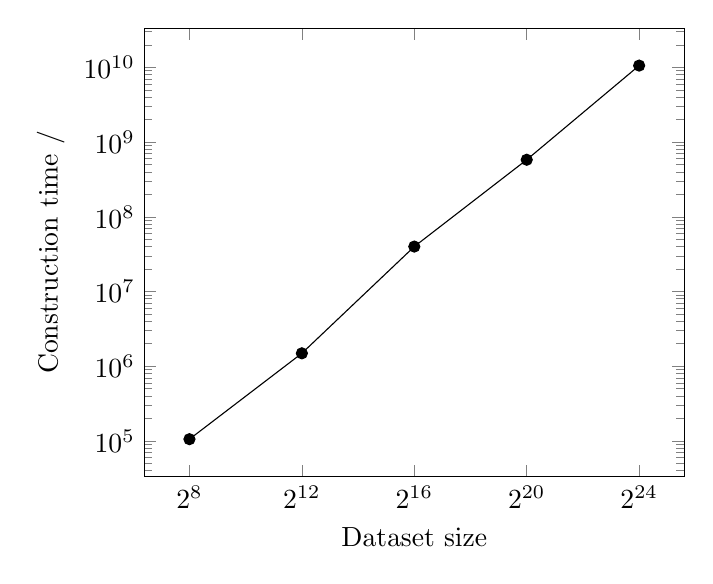
\begin{tikzpicture}
  \begin{loglogaxis}[
    log basis x = 2,
    log basis y = 10,
    xlabel = {Dataset size},
    xtick = {2^8, 2^12, 2^16, 2^20, 2^24},
    ylabel = {\text{Construction time} / \si{\nano\second}},
  ]
    \addplot [mark=*,black] coordinates {
      (256, 105790)
      (4096, 1490690)
      (65536, 39960390)
      (1048576, 579476090)
      (16777216, 10547981289)
    };
  \end{loglogaxis}
\end{tikzpicture}
%
  \caption{Relationship between dataset size and summary construction time}
  \label{fig:count-sketch-implementation-performance}
\end{figure}

The results of all \num{25}~runs of each of the five performance tests are presented in \cref{tab:count-sketch-implementation-performance}, and the relationship between the size of a dataset and the time taken to construct its summary is shown in \cref{fig:count-sketch-implementation-performance}.
This relationship appears to be linear, which agrees with the analysis given in \cref{subsec:count-sketch-analysis-complexity}.
Since the update operation has constant time complexity per update in the size of the data---not to be confused with its linear time complexity in the number of rows---and one update is performed for every item--weight pair in the dataset, the time complexity associated with performing all the updates given in a dataset is linear in the size of the dataset.



\chapter{The Dyadic Count Sketch}
\label{ch:dyadic-count-sketch}

\section{Overview}
\label{sec:fingerprint-overview}

A fingerprint summary is a type of identification summary; it represents the underlying multiset---which may be very large---of a stream \( \mathcal{S} \) as a single, much smaller hash value.
This allows two fingerprints to be compared for equality in order to determine whether they represent the same multiset~\citep{breslauer11}.
In this context, each datum in the stream is an ordered pair of a non-negative integer item \( x \), and a (positive or negative) integer weight \( w \).
The underlying multiset \( S \) comprises all items \( x \) that appear in the stream, and each weight \( w \) is a summand of the multiplicity of its corresponding item in the multiset.
The universe \( U \) from which items are drawn is the integer interval \( U = \dataintegerinterval{u} = \dataintegerinterval{0, u - 1} \), where \( u - 1 \) is the greatest possible value that may appear in the stream~\citep{cormode20}.
This is formalized in \cref{eq:fingerprint-overview-multiset,eq:fingerprint-overview-multiplicity}.

\begin{gather}
  \label{eq:fingerprint-overview-multiset}
  S = \datamultiset[\big]{x \in \dataintegerinterval{u} \suchthat x \in \datasequence{x, w}} \quad \forall\ \datasequence{x, w} \in \mathcal{S}. \\
  \label{eq:fingerprint-overview-multiplicity}
  \cardinality[\big]{\datamultiset{s \in S \suchthat s = x}} = \smashoperator{\sum_{\datasequence{s, w} \in \mathcal{S}}} \indicator_{\dataset{x}} (s) \cdot w \quad \forall\ x \in S.
\end{gather}

Since a multiset maps items (or indices) to multiplicities, a multiset can be represented as a vector of multiplicities.
This means that the fingerprint summary is a solution to the problem of testing for the equality of vectors or sets.
This is a common task in computer science~\citep{breslauer11}.
For example, simple database queries are frequently used to search relations for tuples with a subset of attributes that exactly match a set of given values.
Another example of this problem in database management is the computation of joins, for which, again, tuples are found that match exactly according to a subset of their attributes~\citep{karp87}.
The hash value maintained by a fingerprint summary could also be used as a checksum for validating the correct transmission of packets of data~\citep{tridgell96}.
Although the fingerprint summary is used primarily to check for equality between multisets, multiple fingerprints could be used to check for similarity, since two sets with a large number of equal subsets are likely to be similar.
The ability to check for similarity between vectors of data is useful for search engines, natural language processing and the computation of diffs between files~\citep{tridgell96}.
Although the fingerprint summary is designed to represent multisets of integers, it can be adapted to handle any arbitrary type of data, including strings, as long as a suitable hash function can be found to map each distinct datum to a unique non-negative integer hash value (see \cref{subsec:fingerprint-analysis-universe}).

A fingerprint \( f \) represents a multiset as a hash value in the integer interval \( \dataintegerinterval{0, p - 1} \), where \( p \) is a prime number greater than the upper bound \( u - 1 \) of the universe.
The hash value is computed using a rolling hash function.
This means that the hash value is easily updated for a new input, given only the old hash value and the new input~\citep{karp87}.
This is similar to the computation of a moving average.
The computation of the hash value requires a base \( \alpha \) that must be drawn uniformly at random from the integer interval \( \dataintegerinterval{1, p - 1} \).
The base can be interpreted as a property of the fingerprint.
Thus, in the following algorithms, the base of a fingerprint \( f \) is represented by the primitive routine \( \base (f) \).
Each of the following algorithms is either adapted from, or designed according to the description of, the corresponding operation in the definitive literature~\citep{cormode20}.


\section{Theory}
\label{sec:dyadic-count-sketch-theory}

\begin{algorithm}
  \caption{The dyadic count sketch initialization operation}
  \label{alg:dyadic-count-sketch-theory-initialize}
  \begin{algorithmic}[1]
  \Out the initial array \( C = \dataarray{0}_{m \times n} \) of counters
  \Constant the number \( m \in \positiveintegers \) of rows in the array; the number \( n \in \positiveintegers \) of columns in the array; the prime number \( p \in \dataset{\phi \in \primes \suchthat \phi > n} \)
  \Local the hash functions \( h_{i} \colon \integers \to \dataintegerinterval{n} \) that each map an item to a position in row~\( i \) of the array; the discriminating hash functions \( g_{i} \colon \integers \to \dataset{-1, +1} \) that each map an item to the sign adjustment of its update in row~\( i \) of the array
  \Function{Initialize}{}
    \State \( C \gets \dataarray{0}_{m \times n} \)
    \ForAll{\( i \in \dataintegerinterval{m} \)}
      \State \( \datasequence{\alpha_{i}, \beta_{i}} \gets \) pick uniformly at random from \( \dataintegerinterval{1, p - 1} \)
      \State \( \hashFunction (C, i) \gets h_{i} \colon x \mapsto ((\alpha_{i} \cdot x + \beta_{i}) \Mod p) \Mod n \)
      \State \( \datasequence{\gamma_{i}, \theta_{i}} \gets \) pick uniformly at random from \( \dataintegerinterval{1, p - 1} \)
      \State \( \discriminatorFunction (C, i) \gets g_{i} \colon x \mapsto 2 \cdot (((\gamma_{i} \cdot x + \theta_{i}) \Mod p) \Mod 2) - 1 \)
    \EndFor
    \State \Return \( C \)
  \EndFunction
\end{algorithmic}

\end{algorithm}

The dyadic count sketch initialization operation is presented in \cref{alg:dyadic-count-sketch-theory-initialize}.
A dyadic count sketch is initialized by creating a \( \lambda \)-tuple \( C \) of count sketches, and a \( (L - \lambda) \)-tuple \( D \) of frequency tables.
For each lower level \( l < \lambda \) of the dyadic structure, a count sketch \( C_{l} \) is initialized according to \cref{alg:count-sketch-theory-initialize} by creating an \( m \times n \) array of counters and setting every element in the array to zero.
The hash functions that map items to positions in the count sketch \( C_{l} \) are assigned to the primitive routine \( \hashFunctions (C_{l}) \), and of these, the hash function corresponding to row~\( i \) of \( C_{l} \) is represented by \( \hashFunction (C_{l}, i) \).
Similarly, the discriminating hash functions that determine whether weights should be subtracted from or added to counters in \( C_{l} \) are represented by \( \discriminatorFunctions (C_{l}) \), and of these, the discriminating hash function corresponding to row~\( i \) of \( C_{l} \) is represented by \( \discriminatorFunction (C_{l}, i) \).
For each upper level \( l \geq \lambda \) of the dyadic structure, the index \( l \) is adjusted to the zero-based index \( l' = l - \lambda \), and a frequency table \( D_{l'} \) is initialized by creating a sequence of length \( u / 2^{l} \) and setting every element to zero.
The dyadic structure is returned as an ordered pair of \( C \) and \( D \).
It is assumed that the size \( u \) of the universe, the number of rows \( m \), the number of columns \( n \) and the prime number \( p > n \) have been selected beforehand, and that from these values, the number of levels \( L = \ceiling{\lg u} \) and the number of lower levels \( \lambda = \floor{\lg (u / (m \cdot n))} + 1 \) have been calculated.

\begin{algorithm}
  \caption{The dyadic count sketch update operation}
  \label{alg:dyadic-count-sketch-theory-update}
  \begin{algorithmic}[1]
  \In the fingerprint \( f \in \dataintegerinterval{0, p - 1} \) to update; the item \( x \in U \) for which to update the fingerprint; the weight \( w \in \integers \) of the update to the item
  \Out the updated fingerprint \( f' \in \dataintegerinterval{0, p - 1} \)
  \Constant the prime number \( p \in \dataset{\phi \in \primes \suchthat \phi > u} \)
  \Function{Update}{\relaxedmath{f}, \relaxedmath{x}, \relaxedmath{w}}
    \State \( f' \gets \Copy f \)
    \State \( \base (f') \gets \base (f) \)
    \State \( f' \gets (f' + w \cdot \base (f')^{x}) \Mod p \)
    \State \Return \( f' \)
  \EndFunction
\end{algorithmic}

\end{algorithm}

The dyadic count sketch update operation is presented in \cref{alg:dyadic-count-sketch-theory-update}.
This operation updates a dyadic count sketch \( \datasequence{C, D} \) so as to include in its summary of the underlying multiset an increase in the multiplicity of item \( x \) by weight \( w \).
For each level \( l \) of the dyadic structure, the item \( x \) is mapped to the index \( \upsilon \in \dataintegerinterval{u / 2^{l}} \) for which \( x \) is a member of the dyadic interval \( \dataintegerinterval{\upsilon \cdot 2^{l}, (\upsilon + 1) \cdot 2^{l} - 1} \).
This is achieved by repeated floor division of \( x \) by two, i.e.\@ \( \upsilon = \floor{x / 2^{l}} \).
If the level is a lower level \( l < \lambda \), the count sketch \( C_{l} \) is updated according to \cref{alg:count-sketch-theory-update} so as to include in its summary an increase in the multiplicity of item \( \upsilon \) by weight \( w \).
If the level is an upper level \( l \geq \lambda \), the index \( l \) is adjusted to the zero-based index \( l' = l - \lambda \), and the frequency table \( D_{l'} \) is updated so as to include an increase in the multiplicity of item \( \upsilon \) by weight \( w \).
This is achieved by adding \( w \) to the value at position~\( \upsilon \) of \( D_{l'} \).
The values of the updated dyadic count sketch \( \datasequence{C', D'} \) are given by \cref{eq:dyadic-count-sketch-theory-update-lower,eq:dyadic-count-sketch-theory-update-upper}.

\begin{alignat}{2}
  \label{eq:dyadic-count-sketch-theory-update-lower}
  (C'_{l})_{i, h_{l, i} (\floor{x / 2^{l}})} &= (C_{l})_{i, h_{l, i} (\floor{x / 2^{l}})} + g_{l, i} \Biggl( \floor[\bigg]{\frac{x}{2^{l}}} \Biggr) \cdot w & \quad &\forall\ \datasequence{l, i} \in \dataintegerinterval{0, \lambda - 1} \times \dataintegerinterval{m}. \\
  \label{eq:dyadic-count-sketch-theory-update-upper}
  (D'_{l - \lambda})_{\floor{x / 2^{l}}} &= (D_{l - \lambda})_{\floor{x / 2^{l}}} + w & \quad &\forall\ l \in \dataintegerinterval{\lambda, L - 1}.
\end{alignat}

\begin{algorithm}
  \caption{The dyadic count sketch merge operation}
  \label{alg:dyadic-count-sketch-theory-merge}
  \begin{algorithmic}[1]
  \In the two fingerprints \( a, b \in \dataintegerinterval{0, p - 1} \) to merge (\( \base (a) = \base (b) \))
  \Out the merged fingerprint \( f \equiv a + b \pmod{p} \in \dataintegerinterval{0, p - 1} \)
  \Constant the prime number \( p \in \dataset{\phi \in \primes \suchthat \phi > u} \)
  \Function{Merge}{\relaxedmath{a}, \relaxedmath{b}}
    \State \( f \gets (a + b) \Mod p \)
    \State \( \base (f) \gets \base (a) \)
    \State \Return \( f \)
  \EndFunction
\end{algorithmic}

\end{algorithm}

Two dyadic count sketches can be merged into one.
This operation allows the dyadic count sketch of a stream to be computed in parallel, i.e.\@ dyadic count sketches of distinct portions of a stream can be computed concurrently and eventually combined in order to obtain the dyadic count sketch of the stream as a whole.
The dyadic count sketch merge operation is presented in \cref{alg:dyadic-count-sketch-theory-merge}.
Merging two dyadic count sketches \( A = \datasequence{G, P} \) and \( B = \datasequence{H, Q} \) into a single dyadic count sketch \( T = \datasequence{C, D} \) involves merging the corresponding pair of summaries from \( A \) and \( B \) at each level \( l \) of the dyadic structure.
For each lower level \( l < \lambda \), the two count sketches \( G_{l} \) and \( H_{l} \) are merged according to \cref{alg:count-sketch-theory-merge} into a single count sketch \( C_{l} \) through simple element-wise addition.
This will only work if the two count sketches have the same size and are computed using the same sequences of hash functions, since the hash functions ensure that the dyadic intervals of \( U \) are mapped to the same positions in both count sketches, and that the same discriminating values are applied to update weights for intervals in corresponding positions.
For each upper level \( l \geq \lambda \) of the dyadic structure, the index \( l \) is adjusted to the zero-based index \( l' = l - \lambda \), and the two frequency tables \( P_{l'} \) and \( Q_{l'} \) are merged into a single frequency table \( D_{l'} \), also through element-wise addition.
This works because each element at position~\( \upsilon \) of a frequency table is simply the sum of all the weights corresponding to \( \upsilon \) with which the table has been updated.
Thus, the merged dyadic count sketch \( T = \datasequence{C, D} \) is equivalent to the dyadic count sketch that would be obtained if all the updates to \( A \) and \( B \) were applied to a single dyadic count sketch.
The values of the merged dyadic count sketch \( \datasequence{C, D} \) are given by \cref{eq:dyadic-count-sketch-theory-merge-lower,eq:dyadic-count-sketch-theory-merge-upper}.

\begin{alignat}{2}
  \label{eq:dyadic-count-sketch-theory-merge-lower}
  (C_{l})_{i, j} &= (G_{l})_{i, j} + (H_{l})_{i, j} & \quad &\forall\ \datasequence{l, i, j} \in \dataintegerinterval{0, \lambda - 1} \times \dataintegerinterval{m} \times \dataintegerinterval{n}. \\
  \label{eq:dyadic-count-sketch-theory-merge-upper}
  (D_{l - \lambda})_{\upsilon} &= (P_{l - \lambda})_{\upsilon} + (Q_{l - \lambda})_{\upsilon} & \quad &\forall\ \upsilon \in \dataintegerinterval[\bigg]{\frac{u}{2^{L - \lambda}}} \quad \forall\ l \in \dataintegerinterval{\lambda, L - 1}.
\end{alignat}

\begin{algorithm}
  \caption{The dyadic count sketch rank query operation}
  \label{alg:dyadic-count-sketch-theory-rank-query}
  \begin{algorithmic}[1]
  \In the ordered pair \( \cramped{T \in \integers^{\lambda \times m \times n} \times \integers^{(L - \lambda) \times u / 2^{\lambda}}} \) to query; the item \( x \in U \) whose approximate rank in the multiset \( S \) to return
  \Out the approximate rank \( r \in \nonnegativeintegers \) of the item in the multiset (\( r \simeq \cardinality{\datamultiset{s \in S \suchthat s < x}} \))
  \Constant the number \( L = \ceiling{\lg u} \) of levels in the dyadic structure; the number \( \lambda = \floor{\lg (u / (m \cdot n))} + 1 \) of lower levels in the dyadic structure; the number \( m \in \positiveintegers \) of rows in the array
  \Local the multiset \( F_{l} \in \integers^{m} \) of approximate frequencies of the preceding item in each level~\( l \)
  \Function{Rank-Query}{\relaxedmath{T}, \relaxedmath{x}}
    \State \( \datasequence{C, D} \gets T \)
    \State \( r \gets 0 \)
    \For{\( l \gets 0 \To (L - 1) \)}
      \If{\( x \) is odd}
        \If{\( l < \lambda \)}
        \State \( F_{l} \gets \varnothing \)
          \ForAll{\( i \in \dataintegerinterval{m} \)}
            \State \( j \gets (\hashFunction (C_{l}, i))(x - 1) \)
            \State \( k \gets (\discriminatorFunction (C_{l}, i))(x - 1) \)
            \State \( F_{l} \gets F_{l} \cup \dataset{k \cdot (C_{l})_{i, j}} \)
          \EndFor
          \State \( r \gets r + \median F_{l} \)
        \Else
          \State \( l' \gets l - \lambda \)
          \State \( r \gets r + (D_{l'})_{x - 1} \)
        \EndIf
      \EndIf
      \State \( x \gets x \Div 2 \)
    \EndFor
    \State \Return \( r \)
  \EndFunction
\end{algorithmic}

\end{algorithm}

The dyadic count sketch rank query operation is presented in \cref{alg:dyadic-count-sketch-theory-rank-query}.
This operation returns an approximation of the zero-based rank of an item \( x \) in the multiset summarized by the dyadic count sketch.
For each level \( l \) of the dyadic structure, the item \( x \) is mapped to the index \( \upsilon \in \dataintegerinterval{u / 2^{l}} \) for which \( x \) is a member of the dyadic interval \( \dataintegerinterval{\upsilon \cdot 2^{l}, (\upsilon + 1) \cdot 2^{l} - 1} \).
This is achieved by repeated floor division of \( x \) by two, i.e.\@ \( \upsilon = \floor{x / 2^{l}} \).
If this interval is a right sibling in the binary tree of the dyadic intervals of \( U \), the approximate frequency of its left sibling is added to a cumulative rank \( r \).
For a lower level \( l < \lambda \) of the dyadic structure, the approximate frequency of the interval is queried from the count sketch \( C_{l} \) according to \cref{alg:count-sketch-theory-query} using the index \( \upsilon - 1 \).
For an upper level \( l < \lambda \) of the dyadic structure, the index \( l \) is adjusted to the zero-based index \( l - \lambda \), and the exact frequency of the interval is the value at position~\( \upsilon - 1 \) of the frequency table \( D_{l'} \).
The final rank \( r \) of the item \( x \) is an approximation of the sum of the multiplicities of all items \( s < x \) in the multiset \( S \)
This is formalized in \cref{eq:dyadic-count-sketch-theory-rank-query}.

\begin{equation}
  \label{eq:dyadic-count-sketch-theory-rank-query}
  r \simeq \cardinality[\big]{\datamultiset{s \in S \suchthat s < x}}.
\end{equation}

\begin{algorithm}
  \caption{The dyadic count sketch quantile query operation}
  \label{alg:dyadic-count-sketch-theory-quantile-query}
  \begin{algorithmic}[1]
  \In the ordered pair \( \cramped{T \in \integers^{\lambda \times m \times n} \times \integers^{(L - \lambda) \times u / 2^{\lambda}}} \) to query; the target rank \( t \in \nonnegativeintegers \) in the multiset \( S \) of the item to return
  \Out the item \( x \in U \) whose approximate rank in the multiset is the target rank (\( t \simeq \cardinality{\datamultiset{s \in S \suchthat s < x}} \))
  \Constant the number \( L = \ceiling{\lg u} \) of levels in the dyadic structure; the number \( \lambda = \floor{\lg (u / (m \cdot n))} + 1 \) of lower levels in the dyadic structure; the number \( m \in \positiveintegers \) of rows in the array
  \Local the cumulative rank \( r \in \nonnegativeintegers \) of the item in the multiset; the approximate frequency \( f_{l} \in \integers \) of the item in each level~\( l \); the multiset \( F_{l} \in \integers^{m} \) of approximate frequencies of the item in each level~\( l \)
  \Function{Quantile-Query}{\relaxedmath{T}, \relaxedmath{t}}
    \State \( \datasequence{C, D} \gets T \)
    \State \( x \gets 0 \)
    \State \( r \gets 0 \)
    \For{\( l \gets (L - 1) \DownTo 0 \)}
      \State \( x \gets 2 \cdot x \) \label{line:dyadic-count-sketch-quantile-query-multiplication}
      \If{\( l \geq \lambda \)}
        \State \( l' \gets l - \lambda \)
        \State \( f_{l} \gets (D_{l'})_{x} \)
      \Else
        \State \( F_{l} \gets \varnothing \)
        \ForAll{\( i \in \dataintegerinterval{m} \)}
          \State \( j \gets (\hashFunction (C_{l}, i))(x) \)
          \State \( k \gets (\discriminatorFunction (C_{l}, i))(x) \)
          \State \( F_{l} \gets F_{l} \cup \dataset{k \cdot (C_{l})_{i, j}} \)
        \EndFor
        \State \( f_{l} \gets \median F_{l} \)
      \EndIf
      \If{\( r + f_{l} < t \)}
        \State \( x \gets x + 1 \)
        \State \( r \gets r + f_{l} \)
      \EndIf
    \EndFor
    \State \Return \( x \)
  \EndFunction
\end{algorithmic}

\end{algorithm}

The dyadic count sketch quantile query operation is presented in \cref{alg:dyadic-count-sketch-theory-quantile-query}.
This operation returns an item \( x \) whose zero-based rank in the multiset summarized by the dyadic count sketch is approximately \( t \).
This item is the leaf of the binary tree of  the dyadic intervals of \( U \) whose computed rank is closest to, but no more than, the target rank \( t \).
Starting from the left root interval \( \dataintegerinterval{0, u / 2 - 1} \), the rank of the current node is computed.
If the rank is less than the target rank \( t \), the right sibling of the current node is visited.
The level immediately below is reached by visiting the left child of the resultant node.
This process is repeated until the resultant node is a leaf \( \dataset{x} \).
The item \( x \) held by this leaf is the item of the multiset \( S \) whose rank is approximately \( t \).
This is formalized in \cref{eq:dyadic-count-sketch-theory-quantile-query}.

\begin{equation}
  \label{eq:dyadic-count-sketch-theory-quantile-query}
  \cardinality[\big]{\datamultiset{s \in S \suchthat s < x}} \simeq t.
\end{equation}


\section{Analysis}
\label{sec:count-sketch-analysis}

\subsection{Accuracy}
\label{subsec:count-sketch-analysis-accuracy}

Recall that, in the context of a count sketch, a stream is a sequence of arbitrary length whose elements are each an ordered pair \( \datasequence{x, w} \) of an integer item \( x \) drawn from the universe \( U \subset \integers \) and a (positive or negative) real-valued weight \( w \).
Thus, the value of the counter \( C_{i, j} \) at position~\( j \) of row~\( i \) is, in terms of the stream \( \mathcal{S} \), the sum of the product of the discriminating value \( g_{i} (x) \) and the weight \( w \) corresponding to \( x \) for each item \( x \) that is mapped to position~\( j \) by the hash function \( h_{i} \), as given by \cref{eq:count-sketch-analysis-accuracy-element-stream}.
Since each weight is a summand of the multiplicity of its corresponding item in the multiset, this can be generalized to a sum over all possible values in the universe \( U \) that are mapped to position~\( i \) by the hash function \( h_{i} \).
This is formalized in \cref{eq:count-sketch-analysis-accuracy-element-universe}, where \( w_{x} \) is the multiplicity of the item \( x \) in the underlying multiset \( S \) of the stream.

\begin{alignat}{2}
  \label{eq:count-sketch-analysis-accuracy-element-stream}
  C_{i, j} &= \smashoperator{\sum_{\substack{\datasequence{x, w} \in \mathcal{S} \\ h_{i} (x) = j}}} g_{i} (x) \cdot w & \quad &\forall\ \datasequence{i, j} \in \dataintegerinterval{m} \times \dataintegerinterval{n}. \\
  \label{eq:count-sketch-analysis-accuracy-element-universe}
  C_{i, j} &= \smashoperator{\sum_{\substack{x \in U \\ h_{i} (x) = j}}} g_{i} (x) \cdot w_{x} & \quad &\forall\ \datasequence{i, j} \in \dataintegerinterval{m} \times \dataintegerinterval{n}, \qquad w_{x} = \cardinality[\big]{\datamultiset{s \in S \suchthat s = x}}.
\end{alignat}

Since each item is mapped to a different position in each row, a collision in one row, regardless of its weight, is unlikely to affect the median value of the counters corresponding to the item~\citep{charikar02,cormode20}.
Additionally, the discriminating hash functions help to spread the collisions evenly above and below the median.
For the following analysis of the accuracy of a count sketch to hold, the hash functions \( h_{i} \colon \integers \to \dataintegerinterval{n} \) and \( g_{i} \colon \integers \to \dataset{-1, +1} \) must be pairwise independent, i.e.\@ the hash values of any pair of keys must be independent random variables and the probability of observing any pair of hash values must be uniform.
The analysis also requires a few standard mathematical tools in order to derive upper bounds on errors.
The Markov inequality given in \cref{eq:count-sketch-analysis-accuracy-markov-inequality} provides an upper bound on the probability that a non-negative random variable \( X \) exceeds some constant multiple \( k \) of its expected value~\citep{mitzenmacher05}.

\begin{equation}
  \label{eq:count-sketch-analysis-accuracy-markov-inequality}
  \probability \bigl( X > k \cdot \expectation (X) \bigr) \leq \frac{1}{k}.
\end{equation}

A standard approach to picking an estimate that is accurate with high probability is to take the median of multiple estimates that are each accurate with at least constant probability.
This works because more accurate estimates are likely to be found towards the middle of the sorted order, surrounded by estimates that are too high or too low.
Thus, it is only possible for the median estimate to be inaccurate if at least half of the estimates are inaccurate.
The Chernoff bound argument given in \cref{eq:count-sketch-analysis-accuracy-chernoff-bound-argument} is derived from the Markov inequality in \cref{eq:count-sketch-analysis-accuracy-markov-inequality} and provides an upper bound on the probability that at least half of \( \bigo{\ln (1 / \delta)} \) estimates are inaccurate, where \( X \) is the sum of the Bernoulli random variables that represent whether each estimate is inaccurate~\citep{mitzenmacher05}.
This can be interpreted as an upper bound on the probability that the median of \( \bigo{\ln (1 / \delta)} \) estimates is an inaccurate final estimate.

\begin{equation}
  \label{eq:count-sketch-analysis-accuracy-chernoff-bound-argument}
  \probability \Biggl( X \geq \bigo[\bigg]{\ln \frac{1}{\delta}} \Biggr) < \delta.
\end{equation}

The frequency estimator \( \hat{w}_{x, i} \) of an item \( x \) maintained in row~\( i \) is \( g_{i} (x) \cdot C_{i, h_{i} (x)} \), where the value of the counter \( C_{i, h_{i} (x)} \) is the sum of \( g_{i} (s) \cdot w_{s} \) for all items \( s \) that are also mapped to the position~\( h_{i} (x) \) in row~\( i \).
Thus, the absolute error \( \absolute{w_{x} - \hat{w}_{x, i}} \) in the estimator is given by \cref{eq:count-sketch-analysis-accuracy-absolute-error}.
This is the absolute value of the sum of \( g_{i} (x) \cdot g_{i} (s) \cdot w_{s} \) for all items \( s \) apart from \( x \) that are mapped to the position~\( h_{i} (x) \) in row~\( i \).

\begin{equation}
  \label{eq:count-sketch-analysis-accuracy-absolute-error}
  \absolute{w_{x} - \hat{w}_{x, i}} = \absolute[\Big]{\smashoperator[r]{\sum_{\substack{s \in U \\ s \neq x}}} \indicator_{\dataset{h_{i} (x)}} \bigl( h_{i} (s) \bigr) \cdot g_{i} (x) \cdot g_{i} (s) \cdot w_{s}}.
\end{equation}

This allows the upper bound on the \( L^{1} \)~error of the estimator to be determined as follows.
First, the expected value of the absolute error is be derived according to \cref{eq:count-sketch-analysis-accuracy-absolute-error-expected-value}.
\begin{subequations}
  \label{eq:count-sketch-analysis-accuracy-absolute-error-expected-value}
  \begin{align}
    \begin{split}
      \expectation \bigl( \absolute{w_{x} - \hat{w}_{x, i}} \bigr) &= \expectation \biggl( \absolute[\Big]{\smashoperator[r]{\sum_{\substack{s \in U \\ s \neq x}}} \indicator_{\dataset{h_{i} (x)}} \bigl( h_{i} (s) \bigr) \cdot g_{i} (x) \cdot g_{i} (s) \cdot w_{s}} \biggr) \\
      &\leq \smashoperator{\sum_{\substack{s \in U \\ s \neq x}}} \expectation \biggl( \absolute[\Big]{\indicator_{\dataset{h_{i} (x)}} \bigl( h_{i} (s) \bigr) \cdot g_{i} (x) \cdot g_{i} (s) \cdot w_{s}} \biggr),
    \end{split}
    \intertext{
      and because \( \indicator \in \dataset{0, 1} \) and \( g_{i} (x) \cdot g_{i} (s) \in \dataset{-1, +1} \),
    }
    \begin{split}
      \expectation \bigl( \absolute{w_{x} - \hat{w}_{x, i}} \bigr) &= \smashoperator{\sum_{\substack{s \in U \\ s \neq x}}} \expectation \Bigl( \indicator_{\dataset{h_{i} (x)}} \bigl( h_{i} (s) \bigr) \cdot \absolute{w_{s}} \Bigr) \\
      &= \smashoperator{\sum_{\substack{s \in U \\ s \neq x}}} \expectation \Bigl( \indicator_{\dataset{h_{i} (x)}} \bigl( h_{i} (s) \bigr) \Bigr) \cdot \absolute{w_{s}},
    \end{split}
    \intertext{
      and because the hash functions \( h_{i} \) are pairwise independent and map items uniformly to \( \dataintegerinterval{n} \), the probability \( \probability (h_{i} (s) = h_{i} (x)) \) of collision between \( x \) and \( s \) is \( 1 / n \).
      Thus,
    }
    \begin{split}
      \expectation \bigl( \absolute{w_{x} - \hat{w}_{x, i}} \bigr) &= \frac{1}{n} \cdot \smashoperator{\sum_{\substack{s \in U \\ s \neq x}}} \absolute{w_{s}} \\
      &\leq \frac{\lnorm{1}{\mathvector{w}}}{n},
    \end{split}
  \end{align}
\end{subequations}
where \( \lnorm{1}{\mathvector{w}} \) is the \( L^{1} \)~norm of the vector \( \mathvector{w} \) of multiplicities \( w_{s} \) in the multiset \( S \) for all items \( s \in U \).
By applying the Markov inequality given in \cref{eq:count-sketch-analysis-accuracy-markov-inequality} to the absolute error \( \absolute{w_{x} - \hat{w}_{x, i}} \), it is shown that the error in the estimate exceeds \( k \cdot \lnorm{1}{\mathvector{w}} / n \) with probability at most \( 1 / k \), or rather that the error is at most \( k \cdot \lnorm{1}{\mathvector{w}} / n \) with probability at least \( 1 - 1 / k \).
This is formalized in \cref{eq:count-sketch-analysis-accuracy-absolute-error-bound}.

\begin{equation}
  \label{eq:count-sketch-analysis-accuracy-absolute-error-bound}
  \probability \biggl( \absolute{w_{x} - \hat{w}_{x, i}} > k \cdot \frac{\lnorm{1}{\mathvector{w}}}{n} \biggr) \leq \frac{1}{k}.
\end{equation}

According to the Chernoff bound argument given in \cref{eq:count-sketch-analysis-accuracy-chernoff-bound-argument}, taking the median of \( \bigo{\ln (1 / \delta)} \) estimates---where the number of estimates is given by the number of rows \( m \) in the count sketch---reduces the probability of this error to \( \delta \)~\citep{cormode20}.
Thus, a count sketch with \( m = \bigo{\ln (1 / \delta)} \) rows and \( n = \bigo{1 / \varepsilon} \) columns gives estimates whose absolute errors are at most \( \varepsilon \cdot \lnorm{1}{\mathvector{w}} \) with probability at least \( 1 - \delta \).
A similar analysis can be performed to determine the upper bound on the \( L^{2} \)~error of the estimator.
It follows that a count sketch with \( m = \bigo{\ln (1 / \delta)} \) rows and \( n = \bigo{1 / \varepsilon} \) columns gives estimates whose absolute errors are at most \( \absolute{\sqrt{\varepsilon}} \cdot \lnorm{2}{\mathvector{w}} \) with probability at least \( 1 - \delta \)~\citep{cormode20}.
Since both the \( L^{1} \) and \( L^{2} \) error bounds are achieved by the same query operation, the upper bound on the error of the estimate returned is always the lower of the two.

An alternative frequency summary to the count sketch is the count-min sketch.
This has an almost identical construction to that of the count sketch, but instead of applying discriminating hash functions and returning the median estimate, it returns the minimum estimate~\citep{cormode05}.
This gives a sightly better accuracy guarantee by a constant factor that does not affect the space complexity class, as it will only fail if \emph{all} of the estimates exceed the error threshold~\citep{cormode20}.
Unlike the count-min sketch, however, the count sketch returns an unbiased estimator, since its collisions are distributed evenly above and below the median~\citep{charikar02}.
This property is useful in minimizing error when combining the estimates of multiple count sketches, as in the dyadic count sketch (see \cref{ch:dyadic-count-sketch}).

\subsection{Space and Time Complexities}
\label{subsec:count-sketch-analysis-complexity}

A count sketch maintains an \( m \times n \) array and two sets of \( m \) hash functions, where each hash function can be represented by two integer parameters.
Thus, the overall space complexity of a count sketch is \( \bigo{m \cdot n} \).
Substituting the ideal values \( m = \bigo{\ln (1 / \delta)} \) and \( n = \bigo{1 / \varepsilon} \) given in \cref{subsec:count-sketch-analysis-accuracy} results in a space complexity of \( \bigo{\ln (1 / \delta) \cdot 1 / \varepsilon} \).
The error parameters \( \delta \) and \( \varepsilon \) do not relate to the size of the universe, but to the distribution of weight across the universe.
The \( L^{1} \)~error bound is given in terms of the \( L^{1} \)~norm \( \lnorm{1}{\mathvector{w}} \), which is simply the cardinality of the underlying multiset of the stream.
The \( L^{2} \)~error bound is given in terms of the \( L^{2} \)~norm \( \lnorm{2}{\mathvector{w}} \), which is the square root of the sum of squares of the multiplicities in the underlying multiset of the stream.
If the structure of the data is known beforehand, a suitable value of \( \varepsilon \) can be calculated using estimates of the norm.
Of course, if the structure is known in sufficient detail for an accurate estimate to be made, there is likely little need for a sketch at all.
Hence, \( \delta \) and \( \varepsilon \) can simply be given any value that seems reasonable given the available space and desired accuracy of the application.
Since \( \delta \) and \( \varepsilon \) are independent of the size \( \cardinality{U} \) of the universe, the space complexity \( \bigo{\ln (1 / \delta) \cdot 1 / \varepsilon} \) can be considered constant \( \bigo{1} \) in \( \cardinality{U} \).
For sensible values of \( m \) and \( n \), this constant size \( m \cdot n \) should be less than the size \( \bigo{\cardinality{U}} \) of the more traditional solution that simply maintains a hash table or associative array in which each entry is a key--value pair of an item in the universe and its multiplicity in the underlying multiset of the stream.
Indeed, the values of \( m \) and \( n \) are only sensible if this is the case, otherwise the count sketch would use more space than simply storing the entire underlying multiset of the stream, despite being less accurate.

The initialization operation constructs an \( m \times n \) array and sets its values to zero.
Depending on the implementation language, and the exact implementation of its compilers or interpreters, this should have a time complexity no greater than \( \bigo{m \cdot n} \)~\citep{bentley00}.
It then picks hash function parameters for each of the \( m \) rows in \( \bigo{m} \) time.
The update operation updates one counter on each of the \( m \) rows and therefore has linear time complexity \( \bigo{m} \) in the number of rows \( m \).
The merge operation sums each of the \( m \cdot n \) pairs of corresponding counters in two count sketches.
This takes \( \bigo{m \cdot n} \) time.
The query operation retrieves the value of one counter from each of the \( m \) rows in \( \bigo{m} \) time, and then returns the median.
Finding the median first requires the multiset of approximate frequencies \( F \) to be sorted.
Since no comparison sort can have an average time complexity smaller than \( \bigo{m \cdot \log m} \)~\citep{cormen01}, the query operation has linearithmic time complexity \( \bigo{m \cdot \log m} \) in the number of rows \( m \).

As previously mentioned, the values \( m \) and \( n \) are independent of the size \( \cardinality{U} \) of the universe.
Thus, all of the count sketch operations can be considered to have constant time complexity \( \bigo{1} \) in \( \cardinality{U} \).
Nevertheless, the update and query operations have much greater time overheads than those of the equivalent operations on the more traditional hash table or associative array solutions, even for small values of \( m \) and \( n \).
For example, the query operation of the traditional solution would simply access the entry of an item by index or key in constant time \( \bigo{1} \) and return its value.
The benefit of a count sketch, then, is based entirely on the space it saves.


\section{Implementation and Evaluation}
\label{sec:count-sketch-implementation}

In order to facilitate easy implementation in a wide range of languages, including those from the functional programming paradigm, the operations of the count sketch are presented in the pseudocode as free-standing functions that operate on immutable input data structures without side effects.
The Java implementation takes full advantage of the object-oriented programming paradigm, however, and the corresponding methods are instance members of the mutable \lstinline{CountSketch} class, which implements the \lstinline{getFrequency(int)} query method of the \lstinline{FrequencySummary} interface.
Since the count sketch can accept both positive and negative items, the universe of items used in the implementation is defined to be a subset of the full range of the ubiquitous \num{32}~bit signed \lstinline{int} data type.
This allows the implementation to use the same item data type as that of the \lstinline{Fingerprint} (see \cref{sec:fingerprint-implementation}).
For a similar reason, the \lstinline{int} data type is also used to represent weights.
This means that the update methods of the \lstinline{Fingerprint} and the \lstinline{CountSketch} can share the signature \lstinline{update(int, int)}, which is declared in the \lstinline{MultisetSummary} interface.
The only constraint on the prime number is that it must be greater than the number of columns in the reduced array of the data.
Therefore, the prime chosen was the Mersenne prime \( 2^{31} - 1 \), which is the largest value that can be represented by the \lstinline{int} data type.
This allows up to \( 2^{31} - 2 \) columns in the array, although this many columns would never be used in practice as each row would be half the length of the entire universe of items.
Since multiple rows are required to return an accurate median, it would be more efficient in such a case to simply store the exact frequencies of the items.

The pairwise independent hash functions used in each row are implemented by the \lstinline{LinearHashFunction} class, which implements the \lstinline{apply(int)} method of the \lstinline{HashFunction} functional interface.
The constructor of the class takes a prime number \( p \) and a modulus, and draws a pair of linear and constant term coefficients from the interval \( \dataintegerinterval{1, p - 1} \).
For the hash functions that map items to positions in each row, the modulus is the number of columns.
For the discriminating hash functions, the modulus is two.
This produces a hash value in \( \dataset{0, 1} \), which is mapped to \( \dataset{-1, +1} \) via multiplication by two and subtraction of one.
One issue that arises in the implementation of the hash functions is that the remainder operator (\lstinline{\%}) computes the remainder according to \emph{truncated} division rather than \emph{Euclidean} division~\citep{o14}.
This means that it computes the least positive remainder of the integer division of the absolute value of the first argument by the absolute value of the second, and gives the result the sign of the first.
For positive dividends, this is equivalent to the Euclidean definition of the modulo operation, whereas for negative dividends, it produces negative remainders~\citep{boute92}.
Since the hash values are used as indices in an array, the modulo operations performed by the hash functions must return positive remainders.
The solution is to use the \lstinline{Math.floorMod} method, which computes the remainder according to Knuth's \emph{floored} division~\citep{knuth97,o14}.
Although this is not identical to the Euclidean definition, it does return positive remainders for positive divisors.
This replacement method need only be used for the first modulo operation, as it produces a positive dividend for the second modulo operation.

The initialization operation is implemented as a constructor that takes the number of rows and the number of columns to be used in the reduced array.
Since these sizes remain constant after initialization, the reduced array of data and the sequences of hash functions and estimates are implemented as native arrays rather than lists such as the \lstinline{ArrayList} from the Java collections framework.
The median method is implemented as a static method in the \lstinline{Math} utility class.
This sorts a given array and returns the middle element if the number of elements is odd, or the integer part of the arithmetic mean of the middle two elements if the number of elements is even.

The \lstinline{CountSketchAccumulator} class adapts the summary for use in Apache Spark (see \cref{subsec:introduction-structure-library}).
This allowed two types of test to be performed on the implementation of the count sketch.
The first was a test of the accuracy of its query operation.
The second was a test of the relationship between the size of a dataset and the time taken to construct its summary.
All tests were performed on a single machine using an Intel Core i5-9300H CPU with a base clock speed of \SI{2.40}{\giga\hertz}, four physical cores and eight logical processors, and \SI{8}{\gibi\byte} of RAM\@.
For information regarding how to run the tests, see \cref{app:repository}.

A failure in the accuracy of a count sketch occurs when the absolute error in its approximation of the multiplicity of an item exceeds an error bound expressed as a fraction of the \( L^{1} \)~norm \( \lnorm{1}{\mathvector{w}} \) of the vector of multiplicities of the multiset it summarizes.
The error bound considered in the accuracy test is the \( L^{1} \)~error bound given in \cref{subsec:count-sketch-analysis-accuracy}.
This states that a count sketch with \( m = \bigo{\ln (1 / \delta)} \) rows and \( n = \bigo{1 / \varepsilon} \) columns gives estimates whose absolute errors are at most \( \varepsilon \cdot \lnorm{1}{\mathvector{w}} \) with probability at least \( 1 - \delta \).
Since the failure bound \( \delta \) is determined by the number of rows \( m \), it can be verified empirically by varying the number of rows in the reduced array of the data.

Five series of accuracy tests were performed using the numbers of rows \num{3}, \num{5}, \num{7}, \num{9}, and~\num{11}.
Odd numbers of rows were chosen so as to allow the true median of the estimates of each item to be returned.
A fixed width of ten columns was used in all tests.
This corresponds to a relative error of \SI{10}{\percent} of the \( L^{1} \)~norm of the data.
To obtain a representative sample of results, each test was run \num{25}~times.
On each run, an artificial dataset was generated by drawing \( 2^{16} \) pairs of items and weights uniformly at random from the universe of items and the interval of weights, respectively.
This dataset size was chosen as it is large enough to warrant the use of a streaming algorithm, which offers a reduction in space requirements in exchange for less accurate results.
Conversely, it is not so large that the time and space consumed by the test could prevent other tests from being performed.
For a similar reason, a total of \( 2^{16} \) queries were performed on the count sketch constructed from each dataset.
The items chosen to be queried were distributed uniformly over the universe from which items were drawn.
Since the accuracy is independent of the size of this universe, the items could have been drawn from the full range of the \num{32}-bit signed integer data type used to represent items in the implementation.
However, since only \( 2^{16} \)~items would have been drawn from this range, and a different \( 2^{16} \)~items would have been queried, this would not have been a thorough test of the accuracy of the count sketch, as only one multiplicity at most in every \( 2^{16} \) would have been non-zero.
Instead, the universe was chosen to be \( \dataintegerinterval{-2^{16}, 2^{16} - 1} \).
This allowed for up to half of the items queried to have non-zero multiplicities in the dataset.

Although the weights contribute directly to the \( L^{1} \)~norm of the vector of multiplicities, they also contribute directly to the multiplicities and, to roughly the same extent, the absolute errors in their approximations.
Thus, the accuracy is independent of the size of the interval from which weights are drawn.
This allowed the weights to be drawn from a fixed interval \( \dataintegerinterval{-2^{7}, 2^{7} - 1} \), which can be represented as an \num{8}-bit signed integer.
This was small enough that in the unlikely case that all \( 2^{16} \)~items in the dataset were the same, and that their weights were either all the lower bound \( -2^{7} \) or all the upper bound \( 2^{7} - 1 \), the \num{32}-bit signed integer data type used to represent multiplicities in the implementation would not have overflowed.

Using the Apache~Spark stream processing framework, each dataset was read as input and passed one pair at a time to a \lstinline{CountSketchAccumulator}, which constructed a \lstinline{CountSketch} of the multiset.
Apache~Spark was run using one worker thread for each of the eight logical processors of the test machine.
By running the summary construction in parallel, the correctness of the merge operation was also verified.
The summary was queried for approximations of the multiplicities of \( 2^{16} \) items.
Each approximation was compared to the corresponding true multiplicity in the dataset, and its absolute error was calculated.
If this exceeded the expected error bound \( \varepsilon \cdot \lnorm{1}{\mathvector{w}} \), the query was considered to have failed.
Over all the queries of all the runs that used a given number rows, the proportion of failures was calculated.
If this was less than the corresponding failure bound \( \delta \), the series of tests was considered to have passed.

\begin{table}
  \centering
  \caption{Results of the accuracy tests}
  \label{tab:count-sketch-implementation-accuracy}
  \begin{tabular}{
  S[
    table-alignment = right,
    table-format = 4,
  ]
  S[
    table-alignment = right,
    table-format = 1,
  ]
}
  \toprule
  {Weight upper bound} & {Failures} \\
  \midrule
  16 & 0 \\
  64 & 0 \\
  256 & 0 \\
  1024 & 0 \\
  4096 & 0 \\
  \bottomrule
\end{tabular}
%
\end{table}

The results of all \num{25}~runs of each of the five accuracy tests are presented in \cref{tab:count-sketch-implementation-accuracy}.
This includes the number of rows in the reduced array of the data, the upper bound on the probability of exceeding the expected error bound, and the proportion of failures observed.
Every query passed on every run of every test.
This provides an empirical verification of the correctness of both the design of the count sketch, and the upper bounds on the probabilities of errors and failures.
It should be noted that the failure bound of the last test corresponds to odds of approximately one in \num{60}~thousand.
As with the fingerprint summary, performing this many runs was deemed both infeasible and unnecessary (see \cref{sec:fingerprint-implementation}).
The total of \num{125}~runs was sufficient to show that the probability of a failure is low, even for as few as three rows.

The relationship between the size of a dataset and the time taken to construct its summary was tested via performance tests.
Five series of performance tests were performed using dataset sizes of \( 2^{8} \), \( 2^{12} \), \( 2^{16} \), \( 2^{20} \) and~\( 2^{24} \).
For each of the five series, \num{26}~artificial datasets were generated by drawing the corresponding numbers of pairs of items and weights, in the same manner as for the accuracy tests.
Since only the size of the data was varied for these tests, the items were drawn from the full range of the \num{32}-bit signed integer data type, and the weights were drawn from the arbitrary fixed interval \( \dataintegerinterval{-2^{7}, 2^{7} - 1} \).
After all \num{26}~datasets had been generated, the construction of the \lstinline{CountSketch} of each dataset was timed using only a single worker thread.
The execution time was calculated as the positive difference between the values returned by calls to \lstinline{System.nanoTime()} immediately before and immediately after the construction.
Although this method gives nanosecond precision by querying the most precise available system timer~\citep{o14}, it does not necessarily give nanosecond accuracy, since there is no guarantee regarding the frequency with which this value is updated~\citep{lambert08}.
Nevertheless, it can be assumed that, on average, it is accurate to within hundreds of nanoseconds~\citep{kuperberg09}.
The first run of each series of tests was discarded, as this run `warms up' the test architecture by loading process data into memory and, therefore, encounters page faults and cache misses that should not be considered a feature of normal operation~\citep{luo04}.
The median of the remaining \num{25}~runs was calculated.
Since the execution time can vary greatly due to the presence of other processes, the median is more suitable than the mean as a representation of the typical execution time, as it is not so easily skewed by outliers, and remains meaningful after normalization~\citep{fleming86}.
A sixth series of tests was performed using a dataset containing only a single item--weight pair.
The median execution time of this series was taken as an approximation of the fixed overhead associated with starting the test and initializing the summary.
This was subtracted from the median execution times of the other series of tests in order to normalize them such that they represent only the time taken to update the summary for each item--weight pair in the corresponding dataset.

\begin{table}
  \centering
  \caption{Results of the performance tests}
  \label{tab:count-sketch-implementation-performance}
  \begin{tabular}{
  S[
    table-alignment = right,
    table-format = 8,
  ]
  S[
    table-alignment = right,
    table-format = 11,
  ]
  S[
    table-alignment = right,
    table-format = 11,
  ]
}
  \toprule
  {Dataset size} & \multicolumn{2}{c}{Execution time / \si{\nano\second}} \\
  \cmidrule{2-3}
  & {Median} & {Normalized} \\
  \midrule
  1 & 23927624 & 0 \\
  256 & 23971901 & 44277 \\
  4096 & 24566401 & 638777 \\
  65536 & 72955400 & 49027776 \\
  1048576 & 767910300 & 743982676 \\
  16777216 & 13115900199 & 13091972575 \\
  \bottomrule
\end{tabular}
%
\end{table}

\begin{figure}
  \centering
  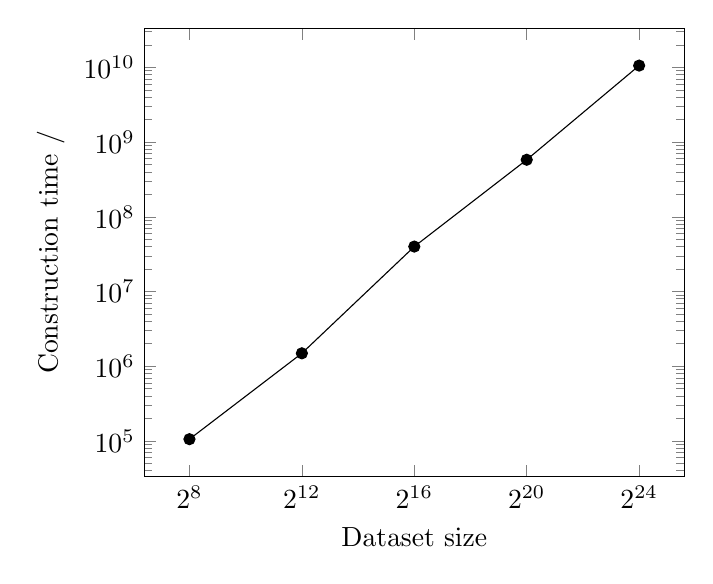
\begin{tikzpicture}
  \begin{loglogaxis}[
    log basis x = 2,
    log basis y = 10,
    xlabel = {Dataset size},
    xtick = {2^8, 2^12, 2^16, 2^20, 2^24},
    ylabel = {\text{Construction time} / \si{\nano\second}},
  ]
    \addplot [mark=*,black] coordinates {
      (256, 105790)
      (4096, 1490690)
      (65536, 39960390)
      (1048576, 579476090)
      (16777216, 10547981289)
    };
  \end{loglogaxis}
\end{tikzpicture}
%
  \caption{Relationship between dataset size and summary construction time}
  \label{fig:count-sketch-implementation-performance}
\end{figure}

The results of all \num{25}~runs of each of the five performance tests are presented in \cref{tab:count-sketch-implementation-performance}, and the relationship between the size of a dataset and the time taken to construct its summary is shown in \cref{fig:count-sketch-implementation-performance}.
This relationship appears to be linear, which agrees with the analysis given in \cref{subsec:count-sketch-analysis-complexity}.
Since the update operation has constant time complexity per update in the size of the data---not to be confused with its linear time complexity in the number of rows---and one update is performed for every item--weight pair in the dataset, the time complexity associated with performing all the updates given in a dataset is linear in the size of the dataset.



\end{document}
